% Generazione delle variabili che andranno a sostituire quelle del template `HomePage.tex`
\newcommand{\documento}{\PdP}
\newcommand{\nomedocumentofisico}{PianoDiProgetto\_v1\_0\_0.pdf}
\newcommand{\redazione}{\TG \\ & \LC}
\newcommand{\verifica}{\NC \\ & \SG \\ & \MM}
\newcommand{\approvazione}{\CV}
\newcommand{\versione}{1.0.0}
\newcommand{\uso}{Esterno}
\newcommand{\destinateTo}{\TV, \\ & \RC, \\ & \II}
\newcommand{\datacreazione}{28 novembre 2018}
\newcommand{\datamodifica}{28 novembre 2018}
\newcommand{\stato}{Approvato}

\def\TABELLE{false}	% abilita - disabilita l'indice delle tabelle
\def\FIGURE{false} 	% abilita - disabilita l'indice delle figure

% Layout del documento 
\documentclass[a4paper,11pt]{article}

\usepackage{ifthen}
\usepackage[english,italian]{babel}
\usepackage[utf8]{inputenc}
\usepackage[T1]{fontenc}
\usepackage{float}
\usepackage{chapterbib}
\usepackage{graphicx}
\usepackage[a4paper,top=2.5cm,bottom=2.5cm,left=2.5cm,right=2.5cm]{geometry}

\PassOptionsToPackage{hyphens}{url}\usepackage[hyperfootnotes=false]{hyperref}
\hypersetup{%
	colorlinks=true,
	citecolor=black,
	linkcolor=black,
	urlcolor=blue
}

\usepackage{enumitem}
\usepackage{eurosym}
\usepackage{booktabs}
\usepackage{fancyhdr}
\usepackage{totpages}
\usepackage{tabularx, array}
\usepackage{dcolumn}
\usepackage{epstopdf}
\usepackage{booktabs}
\usepackage{fancyhdr}
\usepackage{longtable}
\usepackage{calc}
\usepackage{datatool}
\usepackage[bottom]{footmisc}
\usepackage{listings}
\usepackage{textcomp}
\usepackage{titlesec}
\usepackage{rotating}
\usepackage{multirow}
\usepackage{placeins}
\usepackage{color}
\usepackage{makecell}
\usepackage{lscape}
 
\usepackage[table,usenames,dvipsnames]{xcolor}
% Definizione di nuovi colori da poter usare per le tabelle
\definecolor{lightgray}{gray}{0.92}
\definecolor{lightblue}{rgb}{0.93,0.95,1.0}
\definecolor{headgray}{gray}{0.88}

% Ridefinizione dell'env tabularx. Il vecchio è utilizzabile con l'env oldtabularx
\let\oldtabularx\tabularx
\let\endoldtabularx\endtabularx
\renewenvironment{tabularx}{\rowcolors{2}{white}{lightgray}\oldtabularx}{\endoldtabularx}

% Per tabularx con padding, parametro tra [], eg [1.3]
\newenvironment{paddedtablex}[1][1]{%
	\renewcommand*{\arraystretch}{#1}%
	\renewcommand\theadfont{\bfseries}%
	\tabularx%
}{%
	\endtabularx
}

% Ridefinizione dell'env tabular. Il vecchio è utilizzabile con l'env oldtabular
\let\oldtabular\tabular
\let\endoldtabular\endtabular
\renewenvironment{tabular}{\rowcolors{2}{lightgray}{white}\oldtabular}{\endoldtabular}

% Per tabular con padding, parametro tra [], eg [1.3]
\newenvironment{paddedtable}[1][1]{%
	\renewcommand*{\arraystretch}{#1}%
	\renewcommand\theadfont{\bfseries}%
	\tabular%
}{%
	\endtabular
}

% ***TABELLA ANALISI RISCHI PDP***

\newenvironment{risktable}[1][1]{%
	\centering%
	\renewcommand*{\arraystretch}{1.4}%
	\renewcommand\theadfont{\bfseries}%
	\oldtabularx%
}{%
	\endoldtabularx
}

% ***TABELLA SUDDIVISIONE DEL LAVORO PDP***

\newenvironment{detailtable}[1][1]{%
	\centering%
	\renewcommand*{\arraystretch}{1.4}%
	\renewcommand\theadfont{\bfseries}%
	\oldtabularx%
}{%
	\endoldtabularx
}

% ***TABELLA ORGANIGRAMMA***

\newenvironment{orgtable}[1][1]{%
	\centering%
	\renewcommand*{\arraystretch}{1.4}%
	\renewcommand\theadfont{\bfseries}%
	\oldtabularx%
}{%
	\endoldtabularx
}


% DA SPOSTARE SU COMANDI
% ***DOUBLE LINE***

\def\mydoublerule#1#2#3{%%
	\hrule width#1 height#2 \vskip#2
	\hrule width#1 height#3 
}

% ***NUOVO TIPO DI CELLA CENTRATA***

\newcolumntype{Y}{>{\centering\arraybackslash}X}

% ***STILE PAGINA***
\pagestyle{fancy}

% ***INTESTAZIONE***
\rhead{\Large{\progetto} \\ \footnotesize{\documento}}
\lhead{
\includegraphics[keepaspectratio = true, width = 25px]{../template/icons/a6(1).png}}

% ***PIÈ DI PAGINA***
\lfoot{\textit{\gruppo} \\
\footnotesize{\email}}

\rfoot{\thepage} % per le prime pagine: mostra solo il numero romano
\cfoot{}
\renewcommand{\footrulewidth}{0.4pt}   % Linea sopra il piè di pagina
\renewcommand{\headrulewidth}{0.4pt}  % Linea sotto l'intestazione

% ***INSERIMENTO DI NUOVE SOTTOSEZIONI
\setcounter{secnumdepth}{7} %mostra nel documento fino al livello 8 (1.2.3.4.5.6.7.8)
\setcounter{tocdepth}{7}    % mostra nell'indice fino al livello 8 (1.2.3.4.5.6.7.8)


\makeatletter
\newcounter{subsubparagraph}[subparagraph]
\renewcommand\thesubsubparagraph{%
	\thesubparagraph.\@arabic\c@subsubparagraph}
\newcommand\subsubparagraph{%
	\@startsection{subsubparagraph}    % counter
	{6}                              % level
	{\parindent}                     % indent
	{3.25ex \@plus 1ex \@minus .2ex} % beforeskip
	{0.75em}                           % afterskip
	{\normalfont\normalsize\bfseries}}
\newcommand\l@subsubparagraph{\@dottedtocline{6}{10em}{5.5em}} %gestione dell'indice
\newcommand{\subsubparagraphmark}[1]{}
\makeatother

\makeatletter
\newcounter{subsubsubparagraph}[subsubparagraph]
\renewcommand\thesubsubsubparagraph{%
	\thesubsubparagraph.\@arabic\c@subsubsubparagraph}
\newcommand\subsubsubparagraph{%
	\@startsection{subsubsubparagraph}    % counter
	{7}                              % level
	{\parindent}                     % indent
	{3.25ex \@plus 1ex \@minus .2ex} % beforeskip
	{0.75em}                           % afterskip
	{\normalfont\normalsize\bfseries}}
\newcommand\l@subsubsubparagraph{\@dottedtocline{7}{10em}{6.5em}} %gestione dell'indice
\newcommand{\subsubsubparagraphmark}[1]{}
\makeatother


\addtocounter{vZ}{1}
\newcommand{\modifiche}
{
	% \addToDiary{Inserimento qualità di processo}{\Ver}{\NC}{03-01-2018}
	% \addToDiary{Inserimento qualità di prodotto}{\Ver}{\NC}{30-12-2018}
	% \addToDiary{Inserimento standard ISO 90003}{\Ver}{\NC}{27-12-2018}
	% \addToDiary{Inserimento standard ISO 9126}{\Ver}{\NC}{26-12-2018}
	% \addToDiary{Inserimento standard ISO 15504}{\Ver}{\NC}{23-12-2018}
	
	\addToDiary{Aggiunto appendice \S{C} (mitigazione variazioni)}{\Ver}{\MM}{14-02-2019}

	% 1.Y.Z
	\setcounter{vX}{1}%
	\setcounter{vY}{0}%
	\setcounter{vZ}{0}%

	\addToDiary{Approvazione per il rilascio}{\Res}{\NC}{13-01-2019}

	% 0.2.Z
	\decrvX
	\setcounter{vY}{2}%
	\setcounter{vZ}{0}%

	\addToDiary{Verifica finale}{\Ver}{\MM}{12-01-2019}

    % 0.1.Z
    \decrvY%
	\setcounter{vZ}{2}%

	\addToDiary{Aggiunto appendice ``Valutazioni per il miglioramento''}{\Ver}{\MM}{11-01-2019}
	\addToDiary{Inserito ``Resoconto delle attività di verifica''}{\Ver}{\NC}{08-01-2019}
	\addToDiary{Verifica documento}{\Ver}{\CV}{10-12-2018}

    % 0.0.Z
	\setcounter{vZ}{5}%
	\decrvY%

	\addToDiary{Aggiunto appendice ``Standard di qualità''}{\Ver}{\NC}{03-12-2018}
	\addToDiary{Inserito ``Qualità di processo''}{\Ver}{\NC}{02-12-2018}
	\addToDiary{Inserito ``Qualità di prodotto''}{\Ver}{\TG}{01-12-2018}
	\addToDiary{Aggiunta Introduzione}{\Ver}{\NC}{29-11-2018}
    \addToDiary{Creazione template}{\Red}{\TG}{27-11-2018}
}



% Comandi generali
% Generali
\newcommand{\progetto}{Butterfly}
\newcommand{\gruppo}{AlphaSix}
\newcommand{\email}{alpha.six.unipd@gmail.com}

% Documenti
\newcommand{\AdR}{Analisi dei Requisiti}
\newcommand{\NdP}{Norme di Progetto}
\newcommand{\PdP}{Piano di Progetto}
\newcommand{\SdF}{Studio di Fattibilità}
\newcommand{\PdQ}{Piano di Qualifica}
\newcommand{\VI}{Verbale Interno}
\newcommand{\VE}{Verbale Esterno}
\newcommand{\ST}{Specifica Tecnica}
\newcommand{\DDP}{Definizione di Prodotto}
\newcommand{\MU}{Manuale Utente}
\newcommand{\Gl}{Glossario}
\newcommand{\LdP}{Lettera di Presentazione}
\newcommand{\AdRv}{AnalisiDeiRequisiti v2.0.0}
\newcommand{\NdPv}{NormeDiProgetto v2.0.0}
\newcommand{\PdPv}{PianoDiProgetto v2.0.0}
\newcommand{\PdQv}{PianoDiQualifica v2.0.0}
\newcommand{\SdFv}{StudioDiFattibilità v1.0.0}
\newcommand{\DdPv}{DefinizioneDiprodotto v1.0.0}
\newcommand{\Glv}{Glossario v2.0.0}

% Componenti del gruppo
\newcommand{\LC}{Laura Cameran}
\newcommand{\TG}{Timoty Granziero}
\newcommand{\CV}{Ciprian Voinea}
\newcommand{\SG}{Samuele Gardin}
\newcommand{\NC}{Nicola Carlesso}
\newcommand{\MM}{Matteo Marchiori}

% Ruoli
\newcommand{\RdP}{Responsabile di Progetto}
\newcommand{\Res}{Responsabile}
\newcommand{\Red}{Redattore}
\newcommand{\Amm}{Amministratore}
\newcommand{\Ver}{Verificatore}
\newcommand{\Prog}{Progettista}
\newcommand{\Progr}{Programmatore}
\newcommand{\Ana}{Analista}
\newcommand{\RdPs}{Responsabili di Progetto}
\newcommand{\Ress}{Responsabile}
\newcommand{\Amms}{Amministratori}
\newcommand{\Vers}{Verificatori}
\newcommand{\Progs}{Progettisti}
\newcommand{\Progrs}{Programmatori}
\newcommand{\Anas}{Analisti}

% Professori e proponente
\newcommand{\TV}{Prof. Tullio Vardanega}
\newcommand{\RC}{Prof. Riccardo Cardin}
\newcommand{\LuC}{Luca Cappelletti}
\newcommand{\DZ}{Davide Zanetti}
\newcommand{\II}{Imola Informatica}
\newcommand{\proponente}{Imola Informatica}

% Comando per una nuova riga nella tabella del diario delle modifiche
\newcommand{\specialcell}[2][c]{%
	\begin{tabular}[#1]{@{}c@{}}#2\end{tabular}}

\renewcommand*\sectionmark[1]{\markboth{#1}{}}
\renewcommand*\subsectionmark[1]{\markright{#1}}

% Pediodi di lavoro 
\newcommand{\AR}{Analisi dei Requisiti}
\newcommand{\AD}{Analisi dei Requisiti in Dettaglio}
\newcommand{\PA}{Progettazione Architetturale}
\newcommand{\PD}{Progettazione di Dettaglio}
\newcommand{\CO}{Codifica}
\newcommand{\VV}{Validazione}

% Revisioni
\newcommand{\RR}{Revisione dei Requisiti}
\newcommand{\RP}{Revisione di Progettazione}
\newcommand{\RQ}{Revisione di Qualifica}
\newcommand{\RA}{Revisione di Accettazione}

\newcommand{\myincludegraphics}[2][]{%
	\setbox0=\hbox{\phantom{X}}%
	\vtop{
		\hbox{\phantom{X}}
		\vskip-\ht0
		\hbox{\includegraphics[#1]{#2}}}}

% Ridefinizione linea per le note a piè di pagina
\renewcommand{\footnoterule}{%
  \kern -3pt
  \hrule width \textwidth height 0.4pt
  \kern 2pt
}

\colorlet{punct}{red!60!black}
\definecolor{background}{HTML}{EEEEEE}
\definecolor{delim}{RGB}{20,105,176}
\colorlet{numb}{magenta!60!black}
\lstdefinelanguage{json}{
 	basicstyle=\small\ttfamily,
 	numbers=left,
 	numberstyle=\scriptsize,
 	stepnumber=1,
 	numbersep=8pt,
 	showstringspaces=false,
 	breaklines=true,
 	frame=lines,
 	backgroundcolor=\color{background},
 	literate=
 	*{0}{{{\color{numb}0}}}{1}
 	{1}{{{\color{numb}1}}}{1}
 	{2}{{{\color{numb}2}}}{1}
 	{3}{{{\color{numb}3}}}{1}
 	{4}{{{\color{numb}4}}}{1}
 	{5}{{{\color{numb}5}}}{1}
 	{6}{{{\color{numb}6}}}{1}
 	{7}{{{\color{numb}7}}}{1}
 	{8}{{{\color{numb}8}}}{1}
 	{9}{{{\color{numb}9}}}{1}
 	{:}{{{\color{punct}{:}}}}{1}
 	{,}{{{\color{punct}{,}}}}{1}
 	{\{}{{{\color{delim}{\{}}}}{1}
 	{\}}{{{\color{delim}{\}}}}}{1}
 	{[}{{{\color{delim}{[}}}}{1}
 	{]}{{{\color{delim}{]}}}}{1},
}
\lstset{language=json}
\lstset{literate=%
    {Ö}{{\"O}}1
 	{Ä}{{\"A}}1
 	{Ü}{{\"U}}1
 	{é}{{\"s}}1
 	{è}{{\"e}}1
 	{à}{{\"a}}1
	{ö}{{\"o}}1
}


\definecolor{listinggray}{gray}{0.9}
\definecolor{lbcolor}{rgb}{0.9,0.9,0.9}

\lstset{
  backgroundcolor=\color{lbcolor},
  tabsize=4,
  language=Python,
  captionpos=b,
  frame=single,
  numbers=left,
  numberstyle=\tiny,
  numbersep=5pt,
  breaklines=true,
  showstringspaces=false,
  basicstyle=\footnotesize,
  % identifierstyle=\color{magenta},
  keywordstyle=\bfseries\color[rgb]{0,0,1},
  commentstyle=\color[rgb]{0,0.6,0},
  stringstyle=\color{red}
}

% \definecolor{mygreen}{rgb}{0,0.6,0}
% \definecolor{mygray}{rgb}{0.5,0.5,0.5}
% \definecolor{mymauve}{rgb}{0.58,0,0.82}

% \lstset{ 
%   backgroundcolor=\color{white},   % choose the background color; you must add \usepackage{color} or \usepackage{xcolor}; should come as last argument
%   basicstyle=\footnotesize,        % the size of the fonts that are used for the code
%   breakatwhitespace=false,         % sets if automatic breaks should only happen at whitespace
%   breaklines=true,                 % sets automatic line breaking
%   captionpos=b,                    % sets the caption-position to bottom
%   commentstyle=\color{mygreen},    % comment style
%   deletekeywords={...},            % if you want to delete keywords from the given language
%   escapeinside={\%*}{*)},          % if you want to add LaTeX within your code
%   extendedchars=true,              % lets you use non-ASCII characters; for 8-bits encodings only, does not work with UTF-8
%   firstnumber=1000,                % start line enumeration with line 1000
%   frame=single,	                   % adds a frame around the code
%   keepspaces=true,                 % keeps spaces in text, useful for keeping indentation of code (possibly needs columns=flexible)
%   keywordstyle=\color{blue},       % keyword style
%   language=Octave,                 % the language of the code
%   morekeywords={*,...},            % if you want to add more keywords to the set
%   numbers=left,                    % where to put the line-numbers; possible values are (none, left, right)
%   numbersep=5pt,                   % how far the line-numbers are from the code
%   numberstyle=\tiny\color{mygray}, % the style that is used for the line-numbers
%   rulecolor=\color{black},         % if not set, the frame-color may be changed on line-breaks within not-black text (e.g. comments (green here))
%   showspaces=false,                % show spaces everywhere adding particular underscores; it overrides 'showstringspaces'
%   showstringspaces=false,          % underline spaces within strings only
%   showtabs=false,                  % show tabs within strings adding particular underscores
%   stepnumber=2,                    % the step between two line-numbers. If it's 1, each line will be numbered
%   stringstyle=\color{mymauve},     % string literal style
%   tabsize=2,	                   % sets default tabsize to 2 spaces
%   title=\lstname                   % show the filename of files included with \lstinputlisting; also try caption instead of title
% }

\newcommand{\impl}{\textcolor{Green}{Implementato}}
\newcommand{\implno}{\textcolor{Red}{Non Implementato}}

% G di glossario a pedice, con e senza spazio
\newcommand{\GAlt}{\ped{\tiny{G}}}
\newcommand{\G}{\ped{\tiny{G }}}

% e.g. \gloss{progetto}
\newcommand{\gloss}[1]{%
    {\small \textsc{#1}}\GAlt%
}

% D di documento a pedice, con e senza spazio
% \newcommand{\DAlt}{\ped{\tiny{D}}}
\newcommand{\D}{\ped{\tiny{D}}}

% e.g. \Doc{Norme di Progetto}
\newcommand{\Doc}[1]{\textit{#1}\D}

% Comandi per applicare \Doc con un comando unico
\newcommand{\PdQd}{\Doc{\PdQv}}
\newcommand{\PdPd}{\Doc{\PdPv}}
\newcommand{\NdPd}{\Doc{\NdPv}}
\newcommand{\AdRd}{\Doc{\AdRv}}
\newcommand{\SdFd}{\Doc{\SdFv}}
\newcommand{\Gld}{\Doc{\Gld}}

% Le sottosezioni paragraph, subparagraph ecc.. vengono visualizzate come section
\titleformat{\paragraph}{\normalfont\normalsize\bfseries}{\theparagraph}{1em}{}
\titlespacing*{\paragraph}{0pt}{3.25ex plus 1ex minus .2ex}{1.5ex plus .2ex}

\titleformat{\subparagraph}{\normalfont\normalsize\bfseries}{\thesubparagraph}{1em}{}
\titlespacing*{\subparagraph}{0pt}{3.25ex plus 1ex minus .2ex}{1.5ex plus .2ex}

\titleformat{\subsubparagraph}{\normalfont\normalsize\bfseries}{\thesubsubparagraph}{1em}{}
\titlespacing*{\subsubparagraph}{0pt}{3.25ex plus 1ex minus .2ex}{1.5ex plus .2ex}

\titleformat{\subsubsubparagraph}{\normalfont\normalsize\bfseries}{\thesubsubsubparagraph}{1em}{}
\titlespacing*{\subsubsubparagraph}{0pt}{3.25ex plus 1ex minus .2ex}{1.5ex plus .2ex}


% Indentazione paragrafi rimossa. Per metterla manualmente, precedere il paragrafo con il comando /indent
\newlength\tindent
\setlength{\tindent}{\parindent}
\setlength{\parindent}{0pt}
\renewcommand{\indent}{\hspace*{\tindent}}


% Generazione automatica dei numeri per le versioni
\newcounter{vX} % valore per X in X.Y.Z
\newcounter{vY} % valore per Y in X.Y.Z
\newcounter{vZ} % valore per Z in X.Y.Z
\newcommand{\decrvX}{\addtocounter{vX}{-1}} % Comando per il decremento automatico del counter vZ
\newcommand{\decrvY}{\addtocounter{vY}{-1}} % Comando per decrementare vY
\newcommand{\decrvZ}{\addtocounter{vZ}{-1}} % Comando per decrementare vZ
\newcommand{\addToDiary}[4]{\thevX.\thevY.\thevZ & #1 & #2 & #3 & #4\decrvZ\\} % Comando per generare una riga di diario delle modifiche (\addToDiary{desc}{ruolo}{nominativo}{data})

% Colore righe grigie
\newcommand{\tablegray}{gray!20}

% Stile liste
% \renewcommand\labelitemi{$\circ$} % Bullet, primo livello
% \renewcommand\labelitemii{$\diamond$} % Bullet, primo livello
% \renewcommand\labelitemii{\normalfont\bfseries \textendash} % --, secondo livello
% \renewcommand\labelitemiii{\textasteriskcentered} % *, terzo livello
% \renewcommand\labelitemiv{\textperiodcentered} % ., quarto livello
% \setlist[itemize,2]{label=$\circ$}
% \setlist[itemize,2]{label=$\diamond$}

% Placeholder sui diari
\newcommand{\pl}{Placeholder}

%Comandi per le versioni delle tecnologie
\newcommand{\python}{Python 3.6.7}
\newcommand{\gitlab}{GitLab 11.7}
\newcommand{\redmine}{Redmine 4.0.1}
\newcommand{\kafka}{Apache Kafka 2.12}
\newcommand{\docker}{Docker 18.09}
\newcommand{\telegram}{Telegram (Bot API 4.0)}
\newcommand{\slack}{Slack}
\newcommand{\jenkins}{Jenkins 2.146}




\begin{document}
	
    % Inclusione template HomePage
    \begin{center}

%\includegraphics[width=1em]{../../../Template/icone/LogoGruppo.png}
\begin{large} \textbf{\progetto} \end{large}
%\includegraphics[width=1em]{../../../Template/icone/LogoGruppo.png}
\vspace{0.2em}

\hrule
\vspace{7em}


\includegraphics[keepaspectratio = true, width=5cm]{../template/icons/sotto.png}

%Prima pagina senza intestazione né piè di pagina	
\thispagestyle{empty}

%spazio tra il nome e il logo
\vspace{1.5em}

%Copertina
\begin{center} 
  \begin{Huge}
  {\fontsize{15mm}{20mm}\selectfont \gruppoLink} 
  \end{Huge}
\end{center}

%Le informazioni del documento sono ancorate a fine pagina
\vfill

\begin{Huge} \documento \end{Huge}

\begin{center}
% \textbf{Informazioni sul documento} \\ \vspace{2em}
% \small
\begin{tabular}{r|l}
	\multicolumn{2}{c}{\textbf{Informazioni sul documento} } \\ \hline
	\textbf{Nome Documento} & \nomedocumentofisico \\
	% \textbf{Versione} & \versione \\
	\textbf{Data di Creazione} & \datacreazione \\
	\textbf{Data ultima modifica} & \datamodifica \\
	\textbf{Stato} & \stato \\
	\textbf{Redazione} & \redazione \\
	\textbf{Verifica} & \verifica \\
	\textbf{Approvazione} & \approvazione \\
	\textbf{Uso} & \uso \\
	\textbf{Distribuzione} & \gruppo \\
	\textbf{Destinato a} & \destinateTo \\
	\textbf{Email di riferimento} & \email
\end{tabular}
\end{center}

\normalsize

% Sommario
\textbf{Descrizione} \\
Questo documento fornisce la definizioni di alcuni dei termini apparsi in altri documenti allegati redatti 
da \gruppo\ durante lo svolgimento del progetto Butterfly, con
lo scopo di evitare ogni forma di ambiguit\`a.
 

%\vfill
\end{center}

\clearpage

    % Registro delle modifiche e indice
    % si usa la numerazione romana per gli indici e la tabella delle modifiche
    \pagenumbering{Roman}
    \addtocounter{vZ}{1}
\newcommand{\modifiche}
{
	% \addToDiary{Inserimento qualità di processo}{\Ver}{\NC}{03-01-2018}
	% \addToDiary{Inserimento qualità di prodotto}{\Ver}{\NC}{30-12-2018}
	% \addToDiary{Inserimento standard ISO 90003}{\Ver}{\NC}{27-12-2018}
	% \addToDiary{Inserimento standard ISO 9126}{\Ver}{\NC}{26-12-2018}
	% \addToDiary{Inserimento standard ISO 15504}{\Ver}{\NC}{23-12-2018}
	
	\addToDiary{Aggiunto appendice \S{C} (mitigazione variazioni)}{\Ver}{\MM}{14-02-2019}

	% 1.Y.Z
	\setcounter{vX}{1}%
	\setcounter{vY}{0}%
	\setcounter{vZ}{0}%

	\addToDiary{Approvazione per il rilascio}{\Res}{\NC}{13-01-2019}

	% 0.2.Z
	\decrvX
	\setcounter{vY}{2}%
	\setcounter{vZ}{0}%

	\addToDiary{Verifica finale}{\Ver}{\MM}{12-01-2019}

    % 0.1.Z
    \decrvY%
	\setcounter{vZ}{2}%

	\addToDiary{Aggiunto appendice ``Valutazioni per il miglioramento''}{\Ver}{\MM}{11-01-2019}
	\addToDiary{Inserito ``Resoconto delle attività di verifica''}{\Ver}{\NC}{08-01-2019}
	\addToDiary{Verifica documento}{\Ver}{\CV}{10-12-2018}

    % 0.0.Z
	\setcounter{vZ}{5}%
	\decrvY%

	\addToDiary{Aggiunto appendice ``Standard di qualità''}{\Ver}{\NC}{03-12-2018}
	\addToDiary{Inserito ``Qualità di processo''}{\Ver}{\NC}{02-12-2018}
	\addToDiary{Inserito ``Qualità di prodotto''}{\Ver}{\TG}{01-12-2018}
	\addToDiary{Aggiunta Introduzione}{\Ver}{\NC}{29-11-2018}
    \addToDiary{Creazione template}{\Red}{\TG}{27-11-2018}
}

    % Inserisce il link all'indice
% \addcontentsline{toc}{section}{Indice}

\tableofcontents
\clearpage 

% Se è stata impostata a true la variabile per la lista delle tabelle, la mostra
\ifthenelse{\equal{\TABELLE}{true}} 
{\listoftables}{}

% Se è stata impostata a true la variabile per la lista delle figure, la mostra
\ifthenelse{\equal{\FIGURE}{true}}
{\listoffigures}{}

% Da qui comincia la numerazione normale
\pagenumbering{arabic}
\setcounter{page}{1}

% Imposta il formato di visualizzazione
\rfoot{\thepage~di~\pageref{TotPages}}

    % Sezioni documento
    \newpage
\section{Introduzione} \label{Introduzione}
	
	\subsection{Scopo del documento}
	Questo \gloss{documento} ha l'intento di specificare la \gloss{pianificazione} e l'approccio che \gruppo\ adotterà per portare a termine il \gloss{progetto} Butterfly.
	All'interno vengono illustrate le strategie, le suddivisioni dei compiti, l'utilizzo delle risorse, la gestione dei rischi e le attività secondo le quali il team di sviluppo ha intenzione di lavorare.
	
	
    \subsection{Scopo del prodotto}

%%| Ex Norme di Progetto |%%
% Il prodotto che \gruppo\ si incarica di realizzare è Butterfly: un \gloss{tool} di supporto alle figure di	sviluppo di aziende di software
% (non solamente quella committente). Questo applicativo permette di incanalare le notifiche dei vari strumenti utilizzati nel percorso di
% \gloss{CI/CD} (come \gloss{Redmine}, \gloss{GitLab}, ecc.) di un software e, tramite un \gloss{Broker} (\gloss{Apache Kafka} in questo caso),
% spedirli alla persona interessata tramite canale di comunicazione preferito scelto da quest’ultimo (email, \gloss{Telegram}, \gloss{Slack}, ecc).

% \vspace{1cm}

%%| Ex Analisi dei Requisiti |%%
Lo scopo del \gloss{prodotto} è creare un \gloss{applicativo} per poter gestire i messaggi o le segnalazioni provenienti da diversi prodotti per la realizzazione di software,
come \gloss{Redmine}, \gloss{GitLab} e opzionalmente \gloss{SonarQube}, attraverso un \gloss{Broker} che possa incanalare questi messaggi e distribuirli a strumenti come
\gloss{Telegram}, e-mail e opzionalmente \gloss{Slack}.\par
Il software dovrà inoltre essere in grado di riconoscere il \gloss{Topic} dei messaggi in input per poterli inviare in determinati canali a cui i
destinatari dovranno iscriversi.\par
\`E anche richiesto di creare un canale specifico per gestire le particolari esigenze dell'azienda. Dovrà essere in grado, attraverso la lettura di
particolari	\gloss{metadati}, di reindirizzare i messaggi ricevuti al destinatario più appropriato.

% \vspace{1cm}

%%| Ex Piano di Qualifica |%%
% Il prodotto finale consiste in uno strumento in grado di ricevere messaggi o segnalazioni da vari tipi di servizi per la produzione software chiamati
% \gloss{producer} (e.g. \gloss{GitLab}, \gloss{Redmine} e \gloss{SonarQube}), per poterli poi incanalare verso altri servizi chiamati \gloss{Consumer}
% atti a notificare gli sviluppatori (e.g. \gloss{Slack}, \gloss{Telegram} e Email).\par    
% L'applicazione sarà inoltre capace di organizzare le segnalazioni suddividendole per topic a cui i vari utenti dovranno iscriversi per esserne notificati.
% Nel caso in cui il destinatario dovesse segnalare di non essere disponibile, l'applicativo deve reindirizzare il messaggio verso la persona di competenza
% più prossima. 

% \vspace{1cm}

%%| Ex Piano di Progetto |%%
% Il prodotto che \gruppo\ si incarica di realizzare è Butterfly: un tool di supporto alle figure di sviluppo in aziende che producono software (non
% solamente quella del committente).
% Questo applicativo permette di incanalare le notifiche dei vari strumenti utilizzati nel percorso di \gloss{CI} e \gloss{CD} (come Redmine,
% GitLab, ecc.) di un software e, tramite un \gloss{broker} (\gloss{Apache Kafka} in questo caso), spedirli alla persona interessata tramite
% il canale di comunicazione preferito scelto da quest'ultimo (email, Telegram, Slack, ecc.).


	\subsection{Glossario e documenti esterni}
Al fine di rendere il documento più chiaro possibile, i termini che possono assumere un significato ambiguo o i riferimenti a documenti esterni
avranno delle diciture convenzionali:

\begin{itemize}
    \item \textbf{D}: indica che il termine si riferisce al titolo di un particolare documento (ad esempio \Doc{\PdPv});
    \item \textbf{G}: indica che il termine si riferisce ad una voce riportata nel \Doc{\Glv} (ad esempio \gloss{Redmine}).
\end{itemize}

	\subsection{Riferimenti}
		\subsubsection{Riferimenti Normativi}
			\begin{itemize}
				\item \NdPd
				\item Capitolato d'appalto C1:\\
				\url{https://www.math.unipd.it/~tullio/IS-1/2018/Progetto/C1.pdf}
				\item Vincoli di organigramma e specifiche economiche\\
				\url{https://www.math.unipd.it/~tullio/IS-1/2018/Progetto/RO.html}
				\item The Twelve-Factor App, norme per lo sviluppo di un prodotto software consigliate dall'azienda.\\
				\url{https://12factor.net/}
			\end{itemize}
		
		\subsubsection{Riferimenti Informativi}\label{rifinfo}
			\begin{itemize}
				\item Software Engineering - Ian Sommerville - 10 th Edition (2016)
				\item Slide dell’insegnamento Ingegneria del Software\\
				\url{http://www.math.unipd.it/~tullio/IS-1/2018/}
				\item I sistemi per la gestione dei rischi (presentazione rilasciata dalla Bocconi per la gestione dei rischi).\\
				\url{https://www2.deloitte.com/content/dam/Deloitte/it/Documents/risk/Board\%20Academy\%20Corso\%20C6\%2020\%20dic\%202012\%20SDA\%20Bocconi.pdf}
				\item Fonte Figura \ref{fig:modello_incrementale}:\\
				\url{https://it.wikipedia.org/wiki/Modello_incrementale}
			\end{itemize}
		
	\subsection{Scadenze}\label{Scadenze}
	\gruppo\ ha deciso di rispettare le scadenze indicate dal professor Vardanega, riportate di seguito:
	\begin{itemize}
		\item \textbf{Revisione dei Requisiti}: 21-01-2019
		\item \textbf{Revisione di Progetto}: 15-03-2019
		\item \textbf{Revisione di Qualifica}: 19-04-2019
		\item \textbf{Revisione di Accettazione}: 17-05-2019.
	\end{itemize}
	
	\subsection{Modello di sviluppo} % Usare modello di sviluppo come termine al posto di Ciclo di vita in questo contesto. Vedere #26
	Data la natura del progetto, composto da più parti modulari e con un basso valore di accoppiamento, si è scelto di adottare un \gloss{modello di
	sviluppo} ibrido tra quello a componenti e quello incrementale.
	Essi si adattano particolarmente bene a questo tipo di progetto, in quanto:
	\begin{itemize}
		\item Il modello incrementale prevede ripetizioni identificate come cicli di incremento che verranno ripetute fino a quando il prodotto non arriverà a soddisfare i \gloss{requisiti} richiesti dal cliente
		\item Il modello a componenti è basato sul riuso di unità software che possono avere diverse dimensioni:
		\begin{itemize}
			\item \textbf{System reuse}: un intero sistema, composto da più applicazioni, può essere riusato come parte di un sistema di tanti sistemi % TODO: rivedere la frase
			\item \textbf{Application reuse}: un'applicazione può essere riusata incorporandola in altri sistemi senza apportare cambiamenti, 
				oppure configurandola
			\item \textbf{Component reuse}: i \gloss{componenti} di un'applicazione, che possono essere da sotto-sistemi a singoli oggetti, risiedono
				in un cloud o in server privati e possono essere accessibili tramite \gloss{Application Programming Interface} (API)
			\item \textbf{Object and function reuse}: componenti software che implementano una singola funzione o una classe oggetto. Si 
				possono riusare collegandole con lo sviluppo di nuovo codice. Molte di queste sono liberamente disponibili. 
		\end{itemize}
		Oppure, nel caso in cui le componenti siano così specifiche da essere troppo costoso adattarle ad una nuova situazione,
		è possibile fare "concept reuse", ovvero riusare le idee che stanno alla base del componente (e.g. riusare un \gloss{way of working} o un algoritmo). \par
		In particolare, i benefici che si possono trarre dal riuso sono:
		\begin{itemize}
			\item \textbf{Costo complessivo di sviluppo più basso}: perché il numero di componenti software che devono essere progettati, implementati e validati è minore.
			\item \textbf{Sviluppo accelerato}
			\item \textbf{Aumento dell'affidabilità}: un software che è stato provato e testato in altri sistemi risulta più affidabile di un software appena implementato.
			Buona parte dei suoi difetti di progettazione e implementazione dovrebbero già esser stati individuati e corretti.
			%\item  Ridotto rischio di processo, vero specialmente per grandi componenti software riusate come sottosistemi. È un fattore importante per il Project Manager perché riduce il margine di errore nella stima dei costi di un progetto.
			\item \textbf{Conformità con gli standard}: alcuni standard
			%, come gli interface standard, 
			possono essere implementati come set di componenti riusabili.
		\end{itemize}
		%e prevede che venga riutilizzata una base per lo sviluppo dei vari pezzi che formano il progetto, fra loro indipendenti
	\end{itemize}
	Inizialmente si possono spendere le risorse nella realizzazione di una base di partenza per le componenti, che verrà successivamente sviluppata per ciascun requisito richiesto, rappresentando il nucleo del prodotto finale.
	A tale \gloss{milestone} si potranno integrare le funzionalità secondarie richieste dal cliente insieme ai possibili requisiti impliciti desiderabili presenti nel capitolato. In base alla pianificazione svolta, le risorse disponibili saranno ridistribuite in modo da garantire lo sviluppo completo del prodotto.
	L'immagine che segue rappresenta il modello incrementale e come il progetto viene composto da componenti sviluppati ciascuno secondo cicli con fasi ben definite.
	\begin{figure}[H]
		\centering
		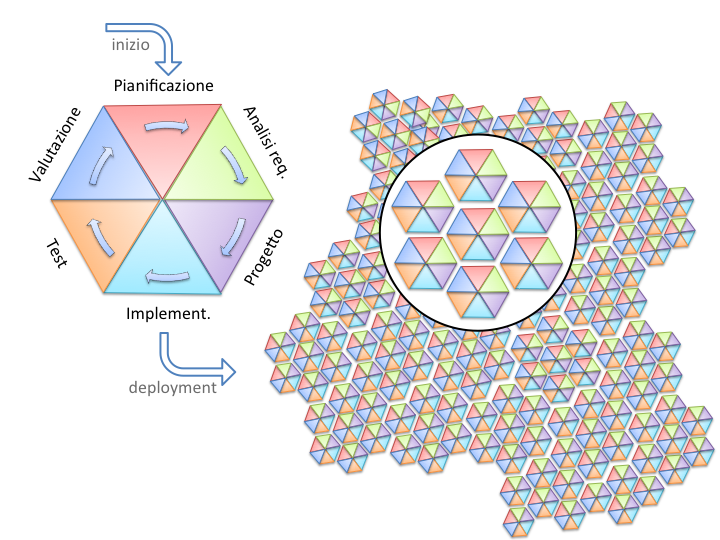
\includegraphics[scale=0.5]{img/modello_incrementale.png}
		\caption{Rappresentazione del modello incrementale\protect\footnotemark}
		\label{fig:modello_incrementale}
	\end{figure}

	\footnotetext{Fonte in \S\ref{rifinfo}}
	 
    
\newpage
\section{Analisi dei rischi} \label{AnalisiDeiRischi}
	Per svolgere un progetto in maniera \gloss{efficiente} ed \gloss{efficace}, viene effettuata un'analisi preliminare dei rischi che potrebbero ostacolare il \gloss{processo} di sviluppo.
	È quindi fondamentale avere un piano di gestione di tali rischi, che permetta di reagire immediatamente in caso dovessero presentarsi, annullandone o limitandone i danni.\\
	I seguenti punti spiegano come è stato deciso di trattare i rischi:
	\begin{itemize}
		\item \textbf{Identificazione}: individuare i potenziali rischi che potrebbero presentarsi.
		\item \textbf{Analisi}: determinare la probabilità di occorrenza e comprenderne la criticità.
		\item \textbf{Pianificazione}: definire strategie che possano evitare i rischi precedentemente incontrati.
		\item \textbf{Controllo}: si monitorano e si revisionano i rischi affinché non si presentino nel corso del progetto.
		\item \textbf{Revisione}: dopo aver risolto eventuali rischi incontrati, si rivede la strategia utilizzata nel caso vengano individuate migliorie per la procedura. Se queste si rivelano più efficaci, vengono applicate.
	\end{itemize}

	\subsection{Valutazione}
	Per la valutazione dei rischi, viene utilizzato uno strumento di misura chiamato Qualitative Risk Assessment che ne considera i criteri quantitativi e qualitativi,
	assegnando a ciascuno un valore di gravità determinato dalla probabilità che il rischio possa avvenire e dalla gravità con cui esso influenza il progetto.
	% VEDI : https://www2.deloitte.com/content/dam/Deloitte/it/Documents/risk/Board%20Academy%20Corso%20C6%2020%20dic%202012%20SDA%20Bocconi.pdf
	Dato il numero non elevato di rischi, si è scelto di mettere solamente tre livelli di gravità e probabilità producendo quindi una matrice con nove elementi. In
	questo modo i rischi possono essere classificati in tre livelli di importanza:

	\begin{itemize}
		\item Basso
		\item Medio
		\item Alto
	\end{itemize}

	\begin{figure}[H]
		\centering
		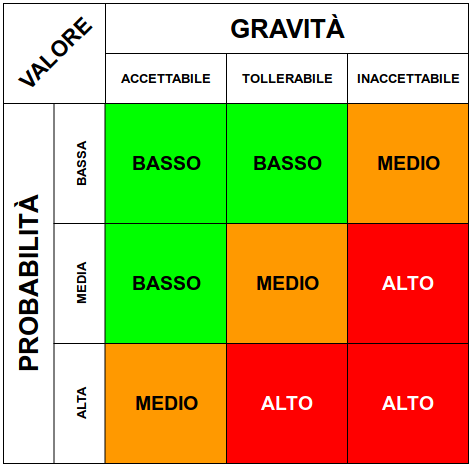
\includegraphics[scale=0.5]{img/risk_assessment_table.png}\\
		\caption{Matrice del Qualitative Risk Assessment}
		\label{fig:rischi}
	\end{figure}

	\subsection{Classificazione}

	A ciascun rischio viene assegnato un codice identificativo in modo da essere univoco e facilmente riconoscibile.

	Questo codice è:

	\begin{center}
		\texttt{[Tipologia][ID]-[Gravità][Probabilità][Classe]}
	\end{center}

	composto da:
	
	\begin{itemize}
		\item \textbf{Tipologia}:
			\begin{itemize}
				\item \textbf{O}: organizzativo.
				\item \textbf{P}: personale.
				\item \textbf{R}: requisiti.
				\item \textbf{S}: strumentale.
				\item \textbf{T}: tecnologico.
			\end{itemize}

		\item \textbf{ID}: numero progressivo di tre cifre che inizia da uno (001 - 999).
		\item \textbf{Gravità}:
			\begin{itemize}
				\item \textbf{0}: accettabile.
				\item \textbf{1}: tollerabile.
				\item \textbf{2}: inaccettabile.
			\end{itemize}

		\item \textbf{Probabilità}:
			\begin{itemize}
				\item \textbf{0}: bassa.
				\item \textbf{1}: media.
				\item \textbf{2}: alta.
			\end{itemize}

		\item \textbf{Classe}: ci si riferisce ai livelli di rischio individuati dalla matrice in Figura \ref{fig:rischi}
			\begin{itemize}
				\item \textbf{0}: basso (verde).
				\item \textbf{1}: medio (arancione).
				\item \textbf{2}: alto (rosso).
			\end{itemize}
	\end{itemize}

	Ad esempio, con P001-021 si può capire, seguendo la legenda, che si tratta del primo rischio del personale, di gravità accettabile, probabilità alta e un valore
	di classe medio.

	\subsection{Lista rischi possibili}

	Per elencare i rischi viene utilizzata una struttura tabellare che indica nella prima riga il codice identificativo e il nome di ciascun rischio,
	mentre nelle righe successive vengono elencate e discusse la relativa descrizione, le strategie per la rilevazione e le eventuali contromisure e mitigazioni.\par

%	Per elencare i rischi viene la seguente struttura tabellare:
%	\begin{table}[H]
%		\begin{risktable}{\columnwidth}{m{1.5cm}m{11.7cm}}
%			\thead{ID} &
%			\thead{Nome significativo}\\
%			\rowcolor{\tablegray}
%			\multicolumn{2}{X}{
%				\thead{Breve descrizione}
%			}\\
%			\multicolumn{2}{X}{
%				\thead{Strategie per la rilevazione}
%			}\\
%			\rowcolor{\tablegray}
%			\multicolumn{2}{X}{
%				\thead{Contromisure e mitigazione}
%			}\\
%		\end{risktable}
%		\caption[Analisi dei rischi]{Struttura della tabella dell'analisi dei rischi}
%	\end{table}

	Dopo un'attenta analisi del capitolato e alcuni incontri tra i componenti del team di sviluppo, è stato deciso di catalogare i seguenti rischi elencandoli in
	maniera crescente rispetto all'ID.
%	\mydoublerule{\linewidth}{0pt}{2pt}
	\begin{table}[H]
		\begin{risktable}{\columnwidth}{m{1.5cm}m{13.5cm}}
			\thead{P001-111} &
			Inesperienza del team a livello tecnico\\
			\rowcolor{\tablegray}
			\multicolumn{2}{X}{
				\textbf{Descrizione}: non tutti i componenti del team hanno le conoscenze di ambienti di sviluppo, linguaggi di programmazione e strumenti richiesti dall'azienda allo stesso livello.
			}\\
			\multicolumn{2}{X}{
				\textbf{Strategia}: sarà compito del \Res\ di progetto parlare con il resto del team di sviluppo e capire le conoscenze di ciascuna delle tecnologie che saranno utilizzate per lo sviluppo del progetto.
			}\\
			\rowcolor{\tablegray}
			\multicolumn{2}{X}{
				\textbf{Mitigazione}: ciascun componente si impegna a sanare le proprie lacune e a portarsi ad un livello comune concordato, in modo da poter lavorare autonomamente e potersi prendere impegni risolvibili senza dover usare tempo ulteriore per imparare la tecnologia.
			}\\
		\end{risktable}
		\caption{Specifica rischio P001-111}
	\end{table}

	\mydoublerule{\linewidth}{0pt}{2pt}

	\begin{table}[H]
		\begin{risktable}{\columnwidth}{m{1.5cm}m{13.5cm}}
			\thead{P002-122} &
			Impreparazione del team a livello gestionale \\
			\rowcolor{\tablegray}
			\multicolumn{2}{X}{
				\textbf{Descrizione}: non avendo affrontato progetti del genere prima d'ora, i componenti di \gruppo\ non conoscono bene i ruoli che devono intraprendere e i compiti da svolgere.
			}\\
			\multicolumn{2}{X}{
				\textbf{Strategia}: sarà compito di chi copre il ruolo di \Res\ assicurarsi che non ci siano perplessità da parte degli altri membri sui ruoli ricoperti e sui compiti assegnati.
			}\\
			\rowcolor{\tablegray}
			\multicolumn{2}{X}{
				\textbf{Mitigazione}: durante le ore di studio personale, ciascun componente si impegnerà a studiare la gerarchia dei ruoli\protect\footnotemark\ e, in caso di dubbi, ne parlerà con il team di sviluppo oppure direttamente con il \Res.
			}\\
		\end{risktable}
		\caption{Specifica rischio P002-122}
	\end{table}

	\footnotetext{Riferirsi alla voce ``Vincoli di organigramma e specifiche economiche'' in \S\ref{rifnorma}}

	\mydoublerule{\linewidth}{0pt}{2pt}

	\begin{table}[H]
		\begin{risktable}{\columnwidth}{m{1.5cm}m{13.5cm}}
			\thead{P003-100} &
			Approvazione errata di documenti \\
			\rowcolor{\tablegray}
			\multicolumn{2}{X}{
				\textbf{Descrizione}: è possibile che il \Res\ commetta errori nella fase di approvazione dei documenti, che potrebbero portare alla consegna di documentazione errata o scadente, causando disguidi con il cliente e lasciando un'impressione negativa. \`E necessario correggere tali sviste, andando quindi a sprecare risorse investibili in altri compiti.
			}\\
			\multicolumn{2}{X}{
				\textbf{Strategia}: il \Res\ deve avere modo di controllare il lavoro prodotto dal proprio team in modo costante e graduale.
			}\\
			\rowcolor{\tablegray}
			\multicolumn{2}{X}{
				\textbf{Mitigazione}: colui che copre il ruolo di \Res\ deve assicurarsi che i documenti approvati siano effettivamente validi; in caso di sviste il \Ver\ deve saper trovare e correggere gli eventuali errori.
			}\\
		\end{risktable}
		\caption{Specifica rischio P003-100}
	\end{table}

	\mydoublerule{\linewidth}{0pt}{2pt}

	\begin{table}[H]

		\begin{risktable}{\columnwidth}{m{1.5cm}m{13.5cm}}
			\thead{P004-100} &
			Cattiva gestione dell'archivio per la documentazione del progetto\\
			\rowcolor{\tablegray}
			\multicolumn{2}{X}{
				\textbf{Descrizione}: data la poca esperienza dei componenti del team di sviluppo con progetti di questo calibro, dove la documentazione è una delle parti principali, gestirla può risultare una novità e potrebbero presentarsi difficoltà nella gestione.
			}\\
			\multicolumn{2}{X}{
				\textbf{Strategia}: l'\Amm\ deve aver predisposto una \gloss{repository} comune in cui ciascun componente possa caricare il proprio lavoro, utilizzandola in maniera tale da non andare a modificare il lavoro caricato dagli altri.
			}\\
			\rowcolor{\tablegray}
			\multicolumn{2}{X}{
				\textbf{Mitigazione}: in caso di errori nella gestione della repository, l'\Amm\ deve saperli risolvere in maniera tempestiva, evitando che chi utilizzi successivamente la repository scarichi file errati, propagando l'errore anche sul proprio sistema.
			}\\
		\end{risktable}
		\caption{Specifica rischio P004-100}
	\end{table}

	\mydoublerule{\linewidth}{0pt}{2pt}

	\begin{table}[H]
		\begin{risktable}{\columnwidth}{m{1.5cm}m{13.5cm}}
			\thead{P005-021} &
			Intesa parziale tra i membri del team di sviluppo\\
			\rowcolor{\tablegray}
			\multicolumn{2}{X}{
				\textbf{Descrizione}: il team di sviluppo è formato principalmente da persone che precedentemente non si conoscevano o che hanno avuto poche interazioni tra di loro fino al momento della creazione di quest'ultimo.
				La mancata conoscenza delle competenze altrui potrebbe causare un'errata gestione del lavoro e dell'assegnazione dei compiti.
			}\\
			\multicolumn{2}{X}{
				\textbf{Strategia}: attraverso gli incontri diretti o con strumenti di chat quali \gloss{Slack}, ci si confronta e si realizzano i diversi modi di lavorare per ognuno.
			}\\
			\rowcolor{\tablegray}
			\multicolumn{2}{X}{
				\textbf{Mitigazione}: il team di sviluppo si impegna a conoscersi nel corso delle riunioni e ritrovi.
				Si discute insieme di un way of working comune che possa soddisfare le metodologie di lavoro di tutti i componenti.
				Nel caso in cui nascano dibattiti o sia difficile raggiungere un punto d'intesa, la decisione è presa dalla maggioranza.
				%e democrazia sia... purtroppo
				%In caso ci fossero dibattiti, per non ricorrere alle lame, gli altri componenti andranno a calmare le acque senza che ci siano morti.
				%LOOOL
			}\\
		\end{risktable}
		\caption{Specifica rischio P005-021}
	\end{table}

	\mydoublerule{\linewidth}{0pt}{2pt}

	\begin{table}[H]

		\begin{risktable}{\columnwidth}{m{1.5cm}m{13.5cm}}
			\thead{P006-122} &
			Cattiva amministrazione delle risorse \\
			\rowcolor{\tablegray}
			\multicolumn{2}{X}{
				\textbf{Descrizione}: data l'inesperienza del team di sviluppo con progetti di questa natura, è possibile che sorgano problemi nell'amministrazione delle risorse come tempo, costi e suddivisione dei ruoli.
			}\\

			\multicolumn{2}{X}{
				\textbf{Strategia}: a ciascuna riunione di \gruppo, si controllerà se il lavoro svolto fino a quel momento è pertinente a quanto è stato preventivato, modificando di conseguenza il consuntivo e il \gloss{preventivo} a finire.
				Tramite strumenti come diagrammi di \gloss{Gantt} dinamici, dove ciascun componente può aggiornare i tempi previsti per completare l'attività assegnata, è possibile monitorare costantemente il progresso del progetto in modo tale da evitare situazioni di \gloss{zero laxity}.
			}\\

			\rowcolor{\tablegray}
			\multicolumn{2}{X}{
				\textbf{Mitigazione}: in caso dovessero sorgere problemi di questa natura, \gruppo\ si impegnerà a ridistribuire le risorse in modo da rispettare la tabella di marcia e in particolar modo le scadenze, tenendo conto di consegnare comunque un prodotto di \gloss{qualità}.
			}\\
		\end{risktable}
		\caption{Specifica rischio P006-122}
	\end{table}

	\mydoublerule{\linewidth}{0pt}{2pt}

	\begin{table}[H]
		\begin{risktable}{\columnwidth}{m{1.5cm}m{13.5cm}}
			\thead{O001-201} &
			Ritardo consegna del materiale per una revisione oltre la scadenza \\
			\rowcolor{\tablegray}
			\multicolumn{2}{X}{
				\textbf{Descrizione}: è possibile che uno o più componenti del team di sviluppo, per impegni legati alla propria vita privata o universitaria, non riescano a gestire i compiti assegnati, arrivando a una scadenza senza aver finito il proprio lavoro e obbligando l'intero team di sviluppo a rinviare la consegna.
			}\\

			\multicolumn{2}{X}{
				\textbf{Strategia}: sarà compito del \Res\ assicurarsi che il lavoro proceda in maniera lineare ponendo scadenze intermedie, monitorando il lavoro del team di sviluppo, organizzando riunioni e aggiornandosi sullo stato dei vari compiti assegnati secondo il way of working scelto.
			}\\

			\rowcolor{\tablegray}
			\multicolumn{2}{X}{
				\textbf{Mitigazione}: ciascun membro si impegna a gestire il proprio tempo adeguatamente in rapporto con gli altri impegni universitari senza trascurare il suo ruolo nel team di sviluppo, distinguendo le priorità in modo da non influenzare negativamente lo sviluppo del progetto. In caso di impegni che possano ostacolare questo obiettivo, ci si prenderà cura di avvisare gli altri componenti del team di sviluppo per tempo.
			}\\
		\end{risktable}
		\caption{Specifica rischio O001-201}	
	\end{table}

	\mydoublerule{\linewidth}{0pt}{2pt}

	\begin{table}[H]
		\begin{risktable}{\columnwidth}{m{1.5cm}m{13.5cm}}
			\thead{O002-010} &
			Mancanza di comunicazione con l'azienda \\

			\rowcolor{\tablegray}
			\multicolumn{2}{X}{
				\textbf{Descrizione}: durante lo sviluppo del progetto, è possibile che non riusciamo a contattare i rappresentanti dell'azienda e che essi quindi non siano al corrente dei progressi fatti, dei requisiti completati e del modo in cui il team sta lavorando.
			}\\

			\multicolumn{2}{X}{
				\textbf{Strategia}: è opportuno che il \Res\ si metta in comunicazione con l'azienda, attraverso \gloss{Telegram}, Skype o tramite incontri di persona e riferisca il progresso svolto dal team di sviluppo, in modo da avere feedback e critiche costruttive che possano migliorare lo sviluppo del progetto.
			}\\

			\rowcolor{\tablegray}
			\multicolumn{2}{X}{
				\textbf{Mitigazione}: in caso di mancata comunicazione per un lungo arco di tempo, è opportuno che alla prima scadenza di revisione utile il team di sviluppo si impegni a contattare l'azienda per avere un suo feedback.
			}\\
		\end{risktable}
		\caption{Specifica rischio O002-010}	
	\end{table}

	\mydoublerule{\linewidth}{0pt}{2pt}

	\begin{table}[H]
		\begin{risktable}{\columnwidth}{m{1.5cm}m{13.5cm}}
			\thead{S001-100} &
			Problematiche hardware \\

			\rowcolor{\tablegray}
			\multicolumn{2}{X}{
				\textbf{Descrizione}: è possibile che i computer e altri strumenti hardware che possono essere utilizzati dai membri del team di sviluppo risultino difettosi o smettano di funzionare.
			}\\

			\multicolumn{2}{X}{
				\textbf{Strategia}: ciascun membro avrà cura degli strumenti a sua disposizione in modo tale che non sorgano problemi che possano ostacolare il lavoro.
			}\\

			\rowcolor{\tablegray}
			\multicolumn{2}{X}{
				\textbf{Mitigazione}: i guasti di natura hardware non sono facilmente prevedibili, ma in caso dovessero presentarsi è possibile utilizzare temporaneamente i computer forniti dai laboratori dell'università fino a quando la macchina difettosa non venga riparata o, se necessario, sostituita.
			}\\
		\end{risktable}
		\caption{Specifica rischio S001-100}		
	\end{table}

	\mydoublerule{\linewidth}{0pt}{2pt}

	\begin{table}[H]

		\begin{risktable}{\columnwidth}{m{1.5cm}m{13.5cm}}
			\thead{R001-122} &
			Interpretazione errata dei requisiti: aggiunta o modifica di requisiti in corso di sviluppo \\

			\rowcolor{\tablegray}
			\multicolumn{2}{X}{
				\textbf{Descrizione}: durante il progetto, dopo aver effettuato una prima analisi di tutti i requisiti, potrebbe sorgere il bisogno di modificare un requisito già fissato o aggiungerne uno non identificato in precedenza.
			}\\

			\multicolumn{2}{X}{
				\textbf{Strategia}: è possibile che nel corso dello sviluppo del progetto vengano scoperti requisiti secondari impliciti non precedentemente valutati che necessitino di essere sviluppati.
				A ciascuna milestone, anche intermedia, è utile controllare che la lista dei requisiti da svolgere sia coerente con quella richiesta dall'azienda, analizzando il documento che presenta il loro capitolato.
			}\\

			\rowcolor{\tablegray}
			\multicolumn{2}{X}{
				\textbf{Mitigazione}: nel caso dovesse sorgere la necessità di sviluppare requisiti non previsti, questi andranno analizzati per capire di che risorse hanno bisogno e come andranno inseriti nella scaletta di sviluppo del progetto in modo adeguato. Data la natura modulare del progetto, ciascun requisito verrà sviluppato in ordine di importanza, in modo da dover svolgere compiti facilmente monitorabili e testabili.
			}\\
		\end{risktable}
		\caption{Specifica rischio R001-122}		
	\end{table}

	\mydoublerule{\linewidth}{0pt}{2pt}

	\begin{table}[H]

		\begin{risktable}{\columnwidth}{m{1.5cm}m{13.5cm}}
			\thead{T001-100} &
			Problematiche software\\

			\rowcolor{\tablegray}
			\multicolumn{2}{X}{
				\textbf{Descrizione}: il team di sviluppo fa affidamento a prodotti software per l'integrazione del codice e dei documenti. Eventuali problemi possono causare gravi perdite di dati.
			}\\

			\multicolumn{2}{X}{
				\textbf{Strategia}: siccome ci si affida a servizi di terze parti, i malfunzionamenti che potrebbero capitare sono imprevedibili, ma data la nota affidabilità di questi strumenti, la probabilità che questo rischio insorga è molto bassa.
			}\\

			\rowcolor{\tablegray}
			\multicolumn{2}{X}{
				\textbf{Mitigazione}: ciascun componente si impegna a mantenere una copia, aggiornata periodicamente, della repository contenente i file di progetto, nella propria macchina o eventualmente in una memoria esterna.
			}\\
		\end{risktable}
		\caption{Specifica rischio T001-100}		
	\end{table}

	\mydoublerule{\linewidth}{0pt}{2pt}
	
	\subsection{Metriche}
	La denominazione delle metriche è presente nel \NdPd.
	
		\subsubsection{MPR008 Rischi non previsti avvenuti}
		Nell'Analisi dei rischi presente nel \Doc{\PdPv}, sono presenti i rischi ritenuti possibili per i quali è proposta una soluzione.
		Possono presentarsi anche rischi non previsti in tale analisi. Questi devono essere il meno possibili (nulli) perché la loro soluzione sarà decisa al momento causando ritardi all'interno del progetto.
		
		\textbf{Metrica}: numero di rischi non previsti avvenuti nel corso dell'intero progetto.

    \newpage
\section{Pianificazione}\label{Pianificazione}
	L'attività di pianificazione consiste nella suddivisione del lavoro tra i vari membri di \gruppo.
	Essa deve fare in modo che ogni componente abbia la possibilità di ricoprire almeno una volta tutti i ruoli di progetto.
    
    Tenendo a mente le scadenze riportate alla sezione \S\ref{Scadenze}, \gruppo\ ha ritenuto opportuno dividere il lavoro in quattro macro-periodi:
	\begin{itemize}
	\item Analisi dei requisiti
	\item Progettazione della base tecnologica
	\item Progettazione di dettaglio e codifica
	\item Validazione e collaudo
	\end{itemize}

	Ogni macro-periodo è stato suddiviso in periodi più brevi (chiamati I periodo, II periodo, etc\dots) per renderne più semplice il
    controllo e la pianificazione. Per esemplificare l'intervallo di tempo tra un macro-periodo e l'altro, verranno usati vari
    diagrammi di Gantt dove sarà chiaro chi ha svolto qualsiasi attività.

    In ognuno di essi ci saranno due milestone (di colore verde):

    \begin{itemize}
    	\item Consegna dei documenti
    	\item Discussione
    \end{itemize}

    \subsection{Analisi dei requisiti}
        Questo macro-periodo ha inizio il 15-11-2018. Procede con quattro periodi fino al 14-01-2019 con la consegna dei documenti e, nel
        quinto e ultimo periodo, \gruppo\ si prepara per la revisione dei requisiti del 21-01-2019.
        
        I ruoli attivi sono:
        \begin{itemize}
            \item Responsabile
            \item Amministratore
            \item Analista
            \item Verificatore
        \end{itemize}
        Questo macro-periodo è stata diviso in cinque periodi:
		\begin{itemize}
			\item \textbf{I periodo}: dal 22-11-2018 al 02-12-2018
			\begin{itemize}
    	        \item \textbf{Discussione capitolati}: sono stati discussi pro e contro di ogni capitolato e, dopo un periodo di
				studio e analisi, \gruppo\ ha concluso con la scelta del capitolato C1.
    	        \item \textbf{Ricerca degli strumenti}: individuazione degli strumenti di supporto da utilizzare durante il progetto.
    	        \item \textbf{Normazione}: definizione di regole per stilare i documenti.
    	        \item \textbf{Distribuzione ruoli e pianificazione attività}
       	        \item \textbf{Studio di fattibilità}
       	        \item \textbf{Pianificazione qualità}: individuazione metodi per garantire qualità del prodotto.
			\end{itemize}
			\newpage
			\item \textbf{II periodo}: dal 03-12-2018 al 16-12-2018
			\begin{itemize}
    	        \item \textbf{Normazione}: definizione di regole per i processi organizzativi.
    	        \item \textbf{Analisi dei rischi}
    	        \item \textbf{Pianificazione qualità}: individuazione dei metodi per garantire qualità del prodotto.
       	        \item \textbf{Ricerca degli strumenti}: individuazione degli strumenti per le varie attività di progetto.
       	        \item \textbf{Pianificazione attività}: diagrammi di Gantt e pianificazione dell'intero progetto.
       	        \item \textbf{Definizione \gloss{casi d'uso}}
			\end{itemize}
        	\item \textbf{III periodo}: dal 17-12-2018 al 29-12-2018
			\begin{itemize}
    	        \item \textbf{Normazione}: definizione di regole per i processi organizzativi.
    	        \item \textbf{Analisi dei requisiti}: ricerca requisiti del capitolato scelto.
       	        \item \textbf{Ricerca degli strumenti}: strumenti per interfacciarsi al \gloss{Producer} e al Broker.
        	\end{itemize}
        	\item \textbf{IV periodo}: dal 30-12-2018 al 13-01-2019
        	\begin{itemize}
       	        \item \textbf{Ricerca degli strumenti}: strumenti per interfacciarsi con il Gestore del personale e con il \gloss{Consumer}.
       	        \item \textbf{Pianificazione attività}: aggiornamenti della pianificazione.
       	        \item \textbf{Stesura lettera di presentazione}
        	\end{itemize}
        	\item \textbf{V periodo}: dal 15-01-2019 al 20-01-2019
        	\begin{itemize}
    	        \item \textbf{Preparazione per la discussione}: realizzazione della presentazione e studio personale.
        	\end{itemize}
		\end{itemize}

        \begin{landscape}
			\subsubsection{Diagramma di Gantt}        
			\begin{figure}[H]
					\centering
					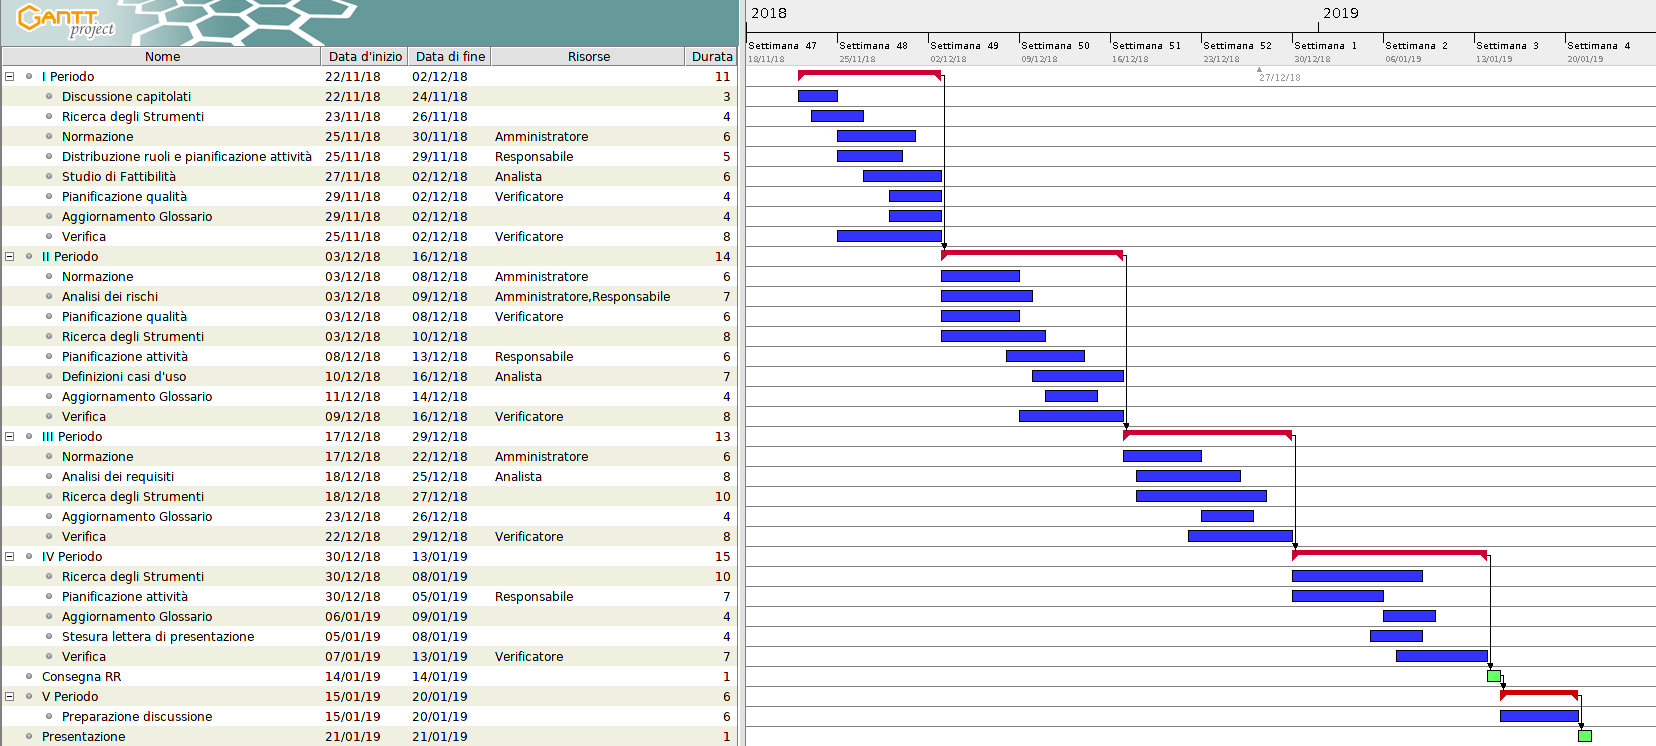
\includegraphics[scale=0.4]{img/Analisi_dei_requisiti.png}\\
					\caption{Diagramma di Gantt della macro analisi dei requisiti}
			\end{figure}
		\end{landscape}
	
		\newpage
		
        \subsection{Progettazione della base tecnologica}
		Questo macro-periodo ha inizio il 22-01-2019, procede con due periodi fino al 08-03-2019 con la consegna
		dei documenti e, nel terzo ed ultimo periodo, \gruppo\ si prepara per la revisione di progetto del 15-03-2019.
        
        I ruoli attivi sono: 
        \begin{itemize}
            \item Responsabile
            \item Amministratore
            \item Analista
            \item Progettista
            \item Programmatore
            \item Verificatore
        \end{itemize}
        Questo macro-periodo è stato suddiviso in tre periodi:
		\begin{itemize}
			\item \textbf{I periodo}: dal 22-01-2019 al 03-02-2019
			\begin{itemize}
    	        \item \textbf{Normazione}
    	        \item \textbf{Analisi dei requisiti}
    	        \item \textbf{Pianificazione delle attività}: aggiornamenti della pianificazione.
    	        \item \textbf{Pianificazione qualità}
    	        \item \textbf{Progettazione}: implementazione schemi \gloss{UML}.
        	\end{itemize}
			\item \textbf{II periodo}: dal 04-02-2019 al 07-03-2019
			\begin{itemize}
				\item \textbf{Ricerca degli strumenti}: \gloss{Apache Kafka}, \gloss{Docker}, \gloss{API Rest}.
    	        \item \textbf{Normazione}: aggiunta nuovi strumenti utilizzati.
    	        \item \textbf{Pianificazione delle attività}: aggiornamenti della pianificazione.
    	        \item \textbf{Progettazione}: implementazione schemi UML.
    	        \item \textbf{Technology Baseline}: tecnologie, \gloss{framework} e librerie per lo sviluppo del prodotto.
    	        \item \textbf{Proof of Concept}: implementazione che rappresenti la \gloss{baseline}.
    	        \item \textbf{Codifica}: realizzazione del \gloss{Proof of Concept}.
    	        \item \textbf{Stesura lettera di presentazione}
        	\end{itemize}
        	\item \textbf{III periodo}: dal 09-03-2019 al 14-03-2019
			\begin{itemize}
				\item \textbf{Preparazione per la discussione}: realizzazione della presentazione e studio personale.
        	\end{itemize}
		\end{itemize}
        
        \begin{landscape}
			\subsubsection{Diagramma di Gantt}        
			\begin{figure}[H]
					\centering
					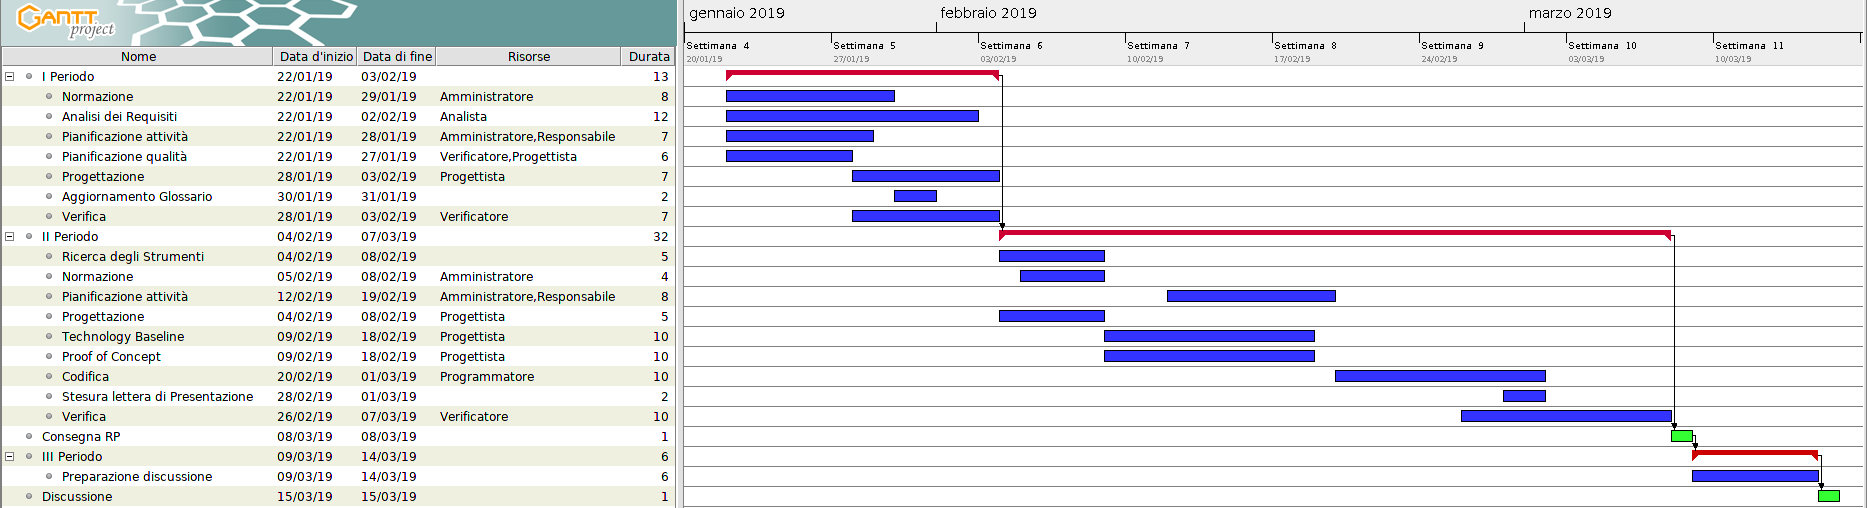
\includegraphics[scale=0.49]{img/Progettazione_della_base_tecnologica.png}\\
					\caption{Diagramma di Gantt della macro progettazione della base tecnologica}
			\end{figure}
		\end{landscape}
		\newpage

        \subsection{Progettazione di dettaglio e codifica}
        Questo macro-periodo ha inizio il 16-03-2019, procede con tre periodi fino al 26-03-2019 con la consegna dei documenti e, nel
        quarto e ultimo periodo, \gruppo\ si prepara per la revisione di qualifica del 19-04-2019.
        
        I ruoli attivi sono: 
        \begin{itemize}
            \item Responsabile
            \item Amministratore
            \item Progettista
            \item Programmatore
            \item Verificatore
        \end{itemize}
        Questo macro-periodo è stato diviso in tre periodi:
		\begin{itemize}
			\item \textbf{I periodo}: dal 16-03-2019 al 26-03-2019
			\begin{itemize}
    	        \item \textbf{Ricerca degli strumenti}
    	        \item \textbf{Pianificazione delle attività}: aggiornamenti della pianificazione.
    	        \item \textbf{Normazione}
    	        \item \textbf{Progettazione}: miglioramento Technology Baseline e Proof of Concept.
    	        \item \textbf{Codifica}: prima implementazione.
        	\end{itemize}
			\item \textbf{II periodo}: dal 27-03-2019 al 03-04-2019
			\begin{itemize}
				\item \textbf{Progettazione e Product Baseline}: implementazione della Product Baseline tramite diagrammi delle classi e di sequenza,
				coerentemente con quanto dichiarato nella Technology Baseline.
    	        \item \textbf{Normazione}
    	        \item \textbf{Codifica}: implementazione seguendo specifiche progettuali ed implementazione dei test.
    	        \item \textbf{Scrittura manuale}: prima stesura.
        	\end{itemize}
        	\item \textbf{III periodo}: dal 04-04-2019 al 11-04-2019
			\begin{itemize}
				\item \textbf{Pianificazione attività}: aggiornamenti della pianificazione.
    	        \item \textbf{Progettazione}: scelta dei \gloss{design pattern}.
    	        \item \textbf{Codifica}: primo rilascio.
    	        \item \textbf{Scrittura manuale}: aggiornamenti al manuale.
    	        \item \textbf{Stesura lettera di presentazione}
        	\end{itemize}
        	\item \textbf{IV periodo}: dal 13-04-2019 al 18-04-2019
			\begin{itemize}
				\item \textbf{Preparazione per la discussione}: realizzazione della presentazione e studio personale.
        	\end{itemize}
        \end{itemize}

        \begin{landscape}
			\subsubsection{Diagramma di Gantt}        
			\begin{figure}[H]
					\centering
					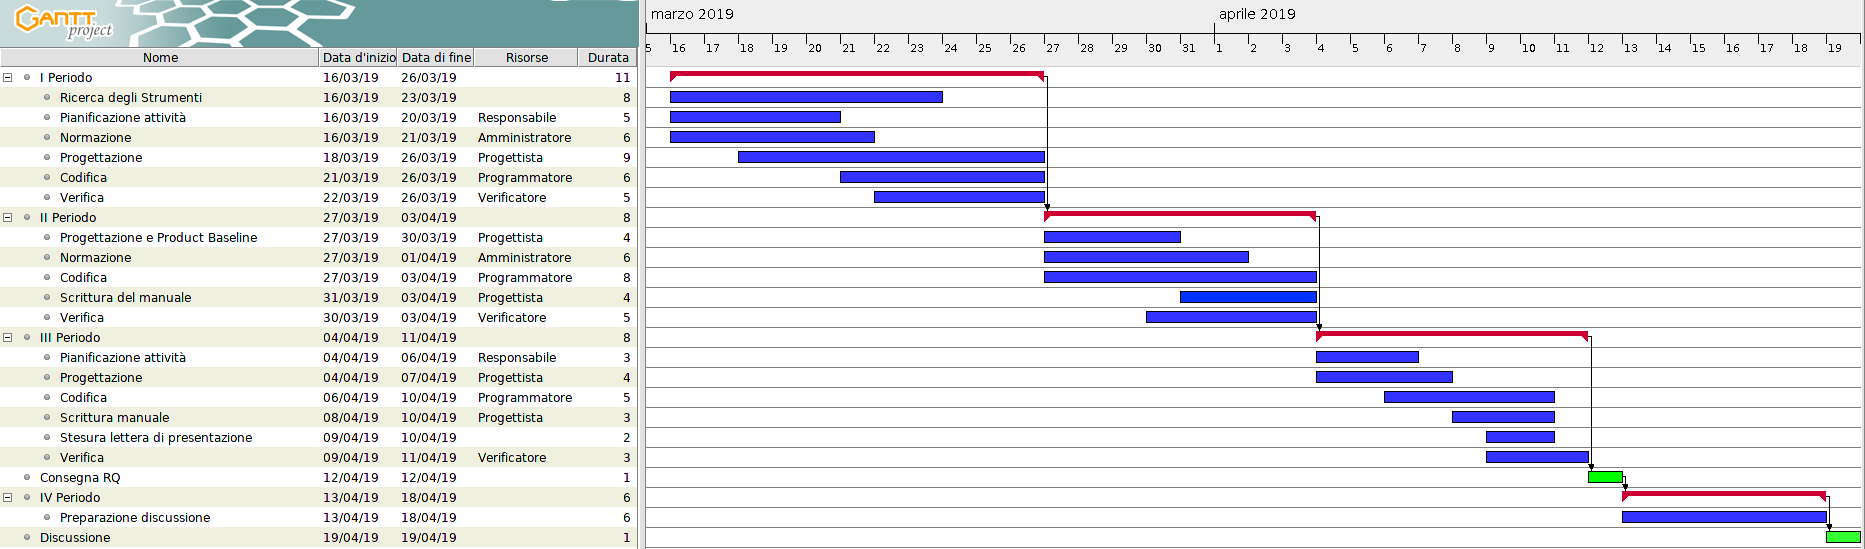
\includegraphics[scale=0.44]{img/Progettazione_di_dettaglio_e_codifica.png}\\
					\caption{Diagramma di Gantt della macro progettazione di dettaglio e codifica}
			\end{figure}
		\end{landscape}
		\newpage

        \subsection{Validazione e collaudo}
        Questo macro-periodo ha inizio il 20-04-2019, procede con due periodi fino al 09-05-2019, con la consegna dei documenti e, nel terzo e ultimo periodo, \gruppo\ si
        prepara per la revisione di accettazione del 17-05-2019.

        I ruoli attivi sono: 
        \begin{itemize}
            \item Amministratore
            \item Analista
            \item Progettista
            \item Programmatore
            \item Verificatore
        \end{itemize}
        Questo macro-periodo è stato diviso in due periodi:
		\begin{itemize}
			\item \textbf{I periodo}: dal 20-04-2019 al 30-04-2019
			\begin{itemize}
    	        \item \textbf{Normazione}
    	        \item \textbf{Analisi dei requisiti}
    	        \item \textbf{Pianificazione attività}: aggiornamenti pianificazione.
    	        \item \textbf{Pianificazione qualità}
    	        \item \textbf{Progettazione Technology Baseline e Product Baseline}: completamento delle specifiche.
        	\end{itemize}
			\item \textbf{II periodo}: dal 01-05-2019 al 09-05-2019
			\begin{itemize}
    	        \item \textbf{Codifica}: completamento ultima versione.
    	        \item \textbf{Scrittura manuale}: completamento manuale.
    	        \item \textbf{Test e collaudo}: esecuzione di test di qualifica e ultimi miglioramenti del prodotto per
    	        garantire che questo soddisfi tutti i vincoli qualitativi.
			\end{itemize}
			\item \textbf{III periodo}: dal 11-05-2019 al 16-05-2019
			\begin{itemize}
				\item \textbf{Preparazione discussione}
			\end{itemize}
		\end{itemize}


        
        \begin{landscape}
			\subsubsection{Diagramma di Gantt}        
			\begin{figure}[H]
					\centering
					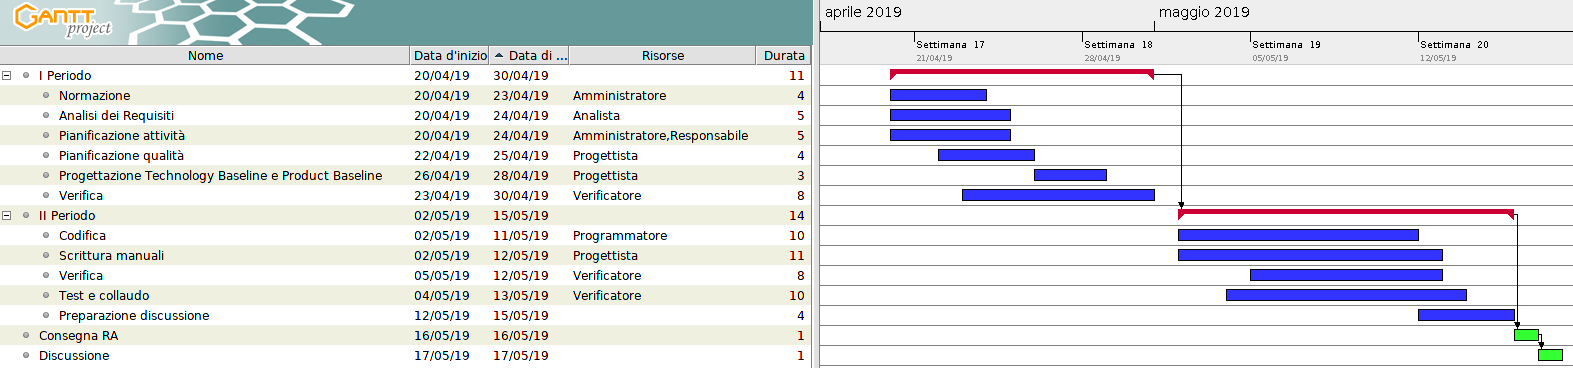
\includegraphics[scale=0.42]{img/Validazione_e_collaudo.png}\\
					\caption{Diagramma di Gantt della macro validazione e collaudo}
			\end{figure}
		\end{landscape}
		\newpage

    % Secondo me da togliere, cade sotto pianificazione (\CV)
    % \newpage
\section{Calendario attivita} \label{CalendarioAttivita}

	Lorem ipsum dolor sit amet, consectetur adipiscing elit, sed do eiusmod tempor incididunt ut labore et dolore magna aliqua. Ut enim ad minim veniam, quis nostrud exercitation ullamco laboris nisi ut aliquip ex ea commodo consequat. Duis aute irure dolor in reprehenderit in voluptate velit esse cillum dolore eu fugiat nulla pariatur. Excepteur sint occaecat cupidatat non proident, sunt in culpa qui officia deserunt mollit anim id est laborum.
	
	\subsection{Consegne}
		\subsubsection{Tabella date}

	Da fare con gantt, vedere anche altri gruppi, sweefty a meno che non sia una cosa fatta nel paragrafo precedente

	Contiene scritto impegno del gruppo a consegare a tot date e per tot scadenze
    \newpage
\section{Suddivisione del lavoro} \label{SuddivisioneDelLavoro}
	
	La sezione riporta la ripartizione dei ruoli tra i membri del team di sviluppo, basandosi su quanto pianificato.
	
	Vengono seguite le seguenti regole:
	\begin{itemize}
		\item ogni membro deve ricoprire ogni ruolo pianificato almeno una volta;
		\item il numero minimo di ore per ruolo che viene ricoperto da un membro in un dato periodo viene fissato a 5 ore;
		\item le ore di lavoro svolte da ogni membro per ogni ruolo dovrà essere più o meno equivalente;
     \end{itemize}
     
     Nel preventivo le ore di lavoro impiegate per la formazione personale non vengono rendicontate.
	
	\newpage
	
	\subsection{Dettaglio Fasi}
		\subsubsection{Analisi dei Requisiti}
			La suddivisione dei ruoli tra i vari membri del team di sviluppo nel periodo di Analisi dei Requisiti è la seguente:
			
			\begin{table}[H]
				\begin{detailtable}{\columnwidth}{m{3cm}YYYYYYY}
					\thead{Membro} & 
					\thead{Re} &
					\thead{Am} &
					\thead{An} &
					\thead{Pj} &
					\thead{Pr} &
					\thead{Ve} &
					\thead{Totale}\\\hline\rowcolor{gray!15}
					Ciprian Voinea & 8 & & 9 & & & 7 & 24\\\hline
					Laura Cameran & & 8 & 9 & & & 7 & 24\\\hline\rowcolor{gray!15}
					Matteo Marchiori & 8 & & 9 & & & 7 & 24\\\hline
					Nicola Carlesso & 8 & & 9 & & & 7 & 24\\\hline\rowcolor{gray!15} 
					Samuele Gardin & & 8 & 9 & & & 7 & 24\\\hline 
					Timoty Graziero & & 8 & 9 & & & 7 & 24
				\end{detailtable}
				\caption{Tabella con la suddivisione oraria nel periodo di Analisi dei Rischi}
			\end{table}
			
			\begin{figure}[H]
					\centering
					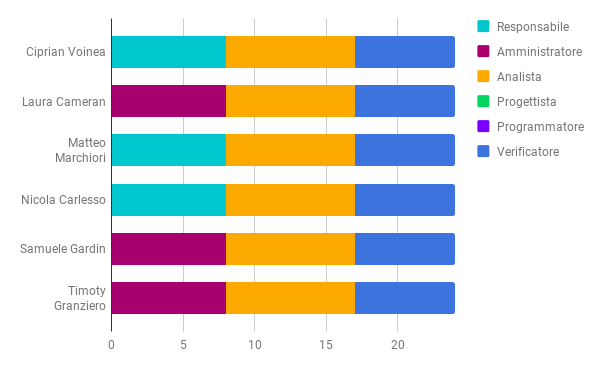
\includegraphics[scale=0.7]{img/Ore_Analisi_dei_Requisiti.png}\\
					\caption{Grafico di suddivisione del lavoro nel periodo di Analisi dei Requisiti}
			\end{figure}
		
		\newpage
		
		\subsubsection{Progettazione della Base Tecnologica}
			La suddivisione dei ruoli tra i vari membri del team di sviluppo nel periodo di Progettazione della Base Tecnologica è la seguente:
			
			\begin{table}[H]
				\begin{detailtable}{\columnwidth}{m{3cm}YYYYYYY}
					\thead{Membro} & 
					\thead{Re} &
					\thead{Am} &
					\thead{An} &
					\thead{Pj} &
					\thead{Pr} &
					\thead{Ve} &
					\thead{Totale}\\\hline\rowcolor{gray!15}
					Ciprian Voinea & & 6 & & 20 & & 14 & 40\\\hline
				    Laura Cameran & 7 & & 7 & 13 & & 23 & 50\\\hline\rowcolor{gray!15}
					Matteo Marchiori & & & & 19 & 23 & 7 & 49\\\hline
					Nicola Carlesso & & 7 & & 20 & 10 & 7 & 44\\\hline\rowcolor{gray!15}
					Samuele Gardin & 8 & & & 13 & 17 & 7 & 45\\\hline
					Timoty Graziero & 7 & 7 & 7 & 15 & & 7 & 43	
				\end{detailtable}
				\caption{Tabella con la suddivisione oraria nel periodo di Progettazione della Base Tecnologica}
			\end{table}
			
			\begin{figure}[H]
					\centering
					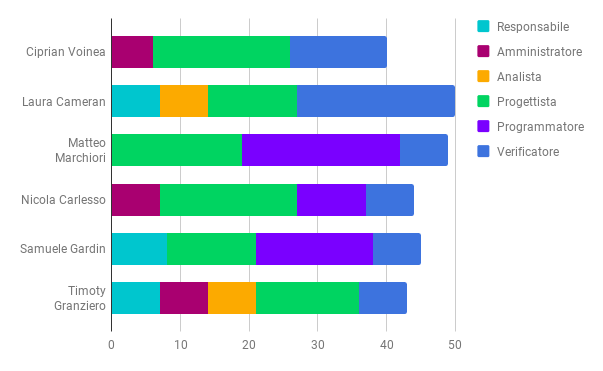
\includegraphics[scale=0.7]{img/Ore_Progettazione_Architetturale.png}\\
					\caption{Grafico di suddivisione del lavoro nel periodo di Progettazione della Base Tecnologica}
			\end{figure}
			
		\newpage
		
		\subsubsection{Progettazione di Dettaglio e Codifica}
			La suddivisione dei ruoli tra i vari membri del team di sviluppo nel periodo di Progettazione di Dettaglio e Codifica è la seguente:
		
			\begin{table}[H]
				\begin{detailtable}{\columnwidth}{m{3cm}YYYYYYY}
					\thead{Membro} & 
					\thead{Re} &
					\thead{Am} &
					\thead{An} &
					\thead{Pj} &
					\thead{Pr} &
					\thead{Ve} &
					\thead{Totale}\\\hline\rowcolor{gray!15}
					Ciprian Voinea & & 6 & & 7 & 20 & 10 & 43\\\hline
					Laura Cameran & 7 & & & 13 & 21 & & 41\\\hline\rowcolor{gray!15}
					Matteo Marchiori & 7 & 6 & & 8 & & 21 & 42\\\hline
					Nicola Carlesso & 8 & & & 7 & 11 & 21 & 47\\\hline\rowcolor{gray!15}
					Samuele Gardin & & 8 & & 16 & & 21 & 45\\\hline
					Timoty Graziero & & & & 14 & 17 & 11 & 42	
				\end{detailtable}
				\caption{Tabella con la suddivisione oraria nel periodo di Progettazione di Dettaglio e Codifica}
			\end{table}
			
			\begin{figure}[H]
					\centering
					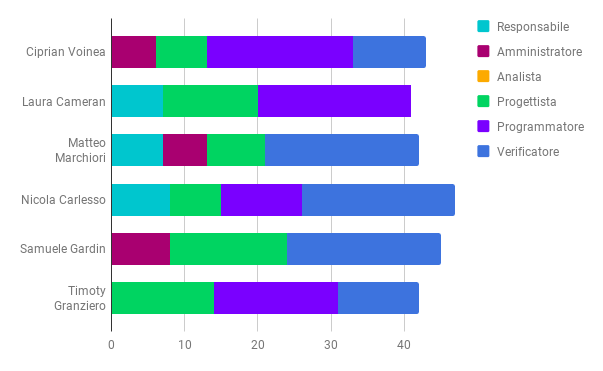
\includegraphics[scale=0.7]{img/Ore_Progettazione_Dettaglio_Codifica.png}\\
					\caption{Grafico di suddivisione del lavoro nel periodo di Progettazione di Dettaglio e Codifica}
			\end{figure}
			
		\newpage
		
		\subsubsection{Validazione e Collaudo}
			La suddivisione dei ruoli tra i vari membri del team di sviluppo nel periodo di Validazione e Collaudo è la seguente:
			
			\begin{table}[H]
				\begin{detailtable}{\columnwidth}{m{3cm}YYYYYYY}
					\thead{Membro} & 
					\thead{Re} &
					\thead{Am} &
					\thead{An} &
					\thead{Pj} &
					\thead{Pr} &
					\thead{Ve} &
					\thead{Totale}\\\hline\rowcolor{gray!15}
					Ciprian Voinea & 8 & & & & & 13 & 21\\\hline
					Laura Cameran & & 5 & & & & 8 & 13\\\hline\rowcolor{gray!15}
					Matteo Marchiori & & 5 & & & & 8 & 13\\\hline
					Nicola Carlesso & & 5 & & & & 8 & 13\\\hline\rowcolor{gray!15}
					Samuele Gardin & 6 & & & & & 8 & 14\\\hline
					Timoty Graziero & 6 & & & & & 13 & 19	
				\end{detailtable}
				\caption{Tabella con la suddivisione oraria nel periodo di Validazione e Collaudo}
			\end{table}
			
			\begin{figure}[H]
					\centering
					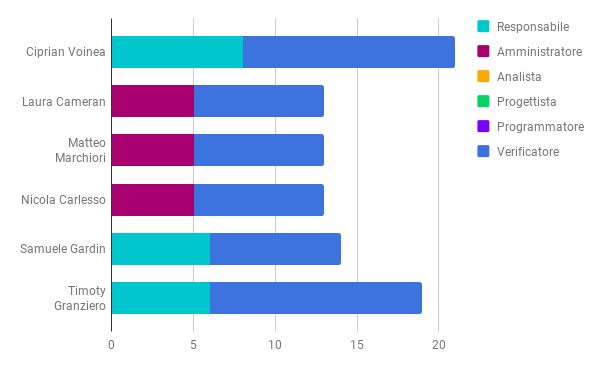
\includegraphics[scale=0.7]{img/Ore_Verifica_Validazione.png}\\
					\caption{Grafico di suddivisione del lavoro nel periodo di Validazione e Collaudo}
			\end{figure}
			
	\newpage

	\subsection{Totali}
		\subsubsection{Ore totali rendicontate}
			Vengono riportate in seguito i totali delle ore rendicontate in preventivo a carico del committente.
			
			\begin{table}[H]
				\begin{detailtable}{\columnwidth}{m{3cm}YYYYYYY}
					\thead{Membro} & 
					\thead{Re} &
					\thead{Am} &
					\thead{An} &
					\thead{Pj} &
					\thead{Pr} &
					\thead{Ve} &
					\thead{Totale}\\\hline\rowcolor{gray!15}
					Ciprian Voinea & 8 & 12 & & 27 & 20 & 37 & 104\\\hline
					Laura Cameran & 14 & 5 & 7 & 26 & 21 & 31 & 104\\\hline\rowcolor{gray!15}
					Matteo Marchiori & 7 & 11 & & 27 & 23 & 36 & 104\\\hline
					Nicola Carlesso & 8 & 12 & & 27 & 21 & 36 & 104\\\hline\rowcolor{gray!15}
					Samuele Gardin & 14 & 8 & & 29 & 17 & 36 & 104\\\hline
					Timoty Graziero & 13 & 7 & 7 & 29 & 17 & 31 & 104	
				\end{detailtable}
				\caption{Tabella con i totali delle ore rendicontate}
			\end{table}
			
			\begin{figure}[H]
					\centering
					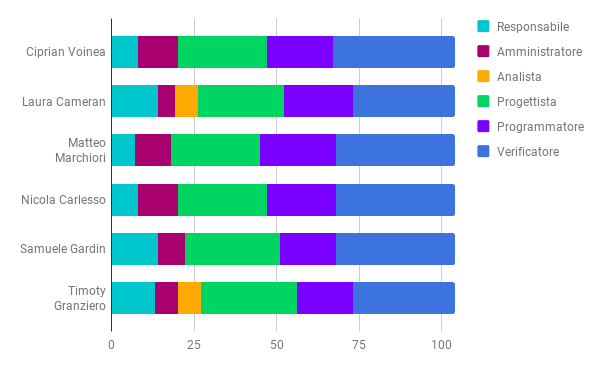
\includegraphics[scale=0.7]{img/Ore_Rendicontate.png}\\
					\caption{Grafico di confronto con le ore rendicontate}
			\end{figure}
		
		\newpage
	
		\subsubsection{Ore totali con investimento}
			Vengono riportate in seguito i totali delle ore rendicontate in preventivo a carico del committente e delle ore di investimento.
			
			\begin{table}[H]
				\begin{detailtable}{\columnwidth}{m{3cm}YYYYYYY}
					\thead{Membro} & 
					\thead{Re} &
					\thead{Am} &
					\thead{An} &
					\thead{Pj} &
					\thead{Pr} &
					\thead{Ve} &
					\thead{Totale}\\\hline\rowcolor{gray!15}
					Ciprian Voinea & 20 & 14 & 11 & 31 & 22 & 46 & 144\\\hline
					Laura Cameran & 18 & 15 & 11 & 30 & 23 & 40 & 144\\\hline\rowcolor{gray!15}
					Matteo Marchiori & 19 & 13 & 11 & 31 & 25 & 45 & 144\\\hline
					Nicola Carlesso & 20 & 14 & 11 & 31 & 23 & 45 & 144\\\hline\rowcolor{gray!15}
					Samuele Gardin & 18 & 18 & 11 & 33 & 19 & 45 & 144\\\hline
					Timoty Graziero & 17 & 17 & 18 & 33 & 19 & 40 & 144	
				\end{detailtable}
				\caption{Tabella con i totali delle ore rendicontate e di investimento}
			\end{table}
			
			\begin{figure}[H]
					\centering
					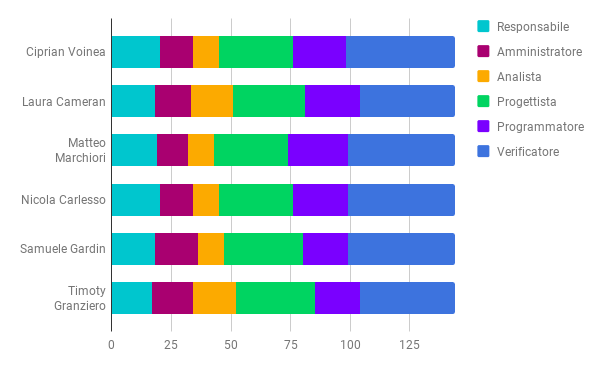
\includegraphics[scale=0.7]{img/Ore_Totali.png}\\
					\caption{Grafico di confronto con le ore totali}
			\end{figure}
    \newpage
\section{Prospetto economico} \label{ProspettoEconomico}
	La sezione riporta il prospetto economico dettagliato rispettante la suddivisione del lavoro stabilita.

	\subsection{Analisi dei requisiti}\label{Analisi dei Requisiti}
		Il prospetto economico relativo al periodo di Analisi dei requisiti è il seguente.
		
		\begin{table}[H]
			\begin{detailtable}{\columnwidth}{m{3cm}YY}
				\thead{Ruolo} & 
				\thead{Totale ore} &
				\thead{Costo in \euro}\\\toprule\rowcolor{\tablegray}
				Responsabile & 24 & 720,00\\
				Amministratore & 24 & 480,00\\\rowcolor{\tablegray}
				Analista & 54 & 1350,00\\
				Progettista & - & - \\\rowcolor{\tablegray}
				Programmatore & - & - \\
				Verificatore & 42 & 630,00\\\rowcolor{\tablegray}
				\textbf{Totale} & \textbf{144} & \textbf{3180,00}\\\bottomrule
			\end{detailtable}
			\caption{Prospetto economico del periodo di Analisi dei requisiti}
		\end{table}

	\subsection{Progettazione della base tecnologica}\label{Progettazione base tecnologica}
		Il prospetto economico relativo al periodo di Progettazione della base tecnologica è il seguente.
		
		\begin{table}[H]
			\begin{detailtable}{\columnwidth}{m{3cm}YY}
				\thead{Ruolo} & 
				\thead{Totale ore} &
				\thead{Costo in \euro}\\\toprule\rowcolor{\tablegray}
				Responsabile & 25 & 750,00\\
				Amministratore & 20 & 400,00\\\rowcolor{\tablegray}
				Analista & 14 & 350,00\\
				Progettista & 52 & 1144,00\\\rowcolor{\tablegray}
				Programmatore & 102 & 1530,00\\
				Verificatore & 67 & 1005,00\\\rowcolor{\tablegray}
				\textbf{Totale} & \textbf{280} & \textbf{5179,00}\\\bottomrule
			\end{detailtable}
			\caption{Prospetto economico del periodo di Progettazione della base tecnologica}
		\end{table}
		
	\newpage
	
	\subsection{Progettazione di dettaglio e codifica}\label{Progettazione di dettaglio e codifica}
		Il prospetto economico relativo al periodo di Progettazione di dettaglio e codifica è il seguente.
		
		\begin{table}[H]
			\begin{detailtable}{\columnwidth}{m{3cm}YY}
				\thead{Ruolo} & 
				\thead{Totale ore} &
				\thead{Costo in \euro}\\\toprule\rowcolor{\tablegray}
				Responsabile & 22 & 660,00\\
				Amministratore & 20 & 400,00\\\rowcolor{\tablegray}
				Analista & - & - \\
				Progettista & 65 & 1430,00\\\rowcolor{\tablegray}
				Programmatore & 69 & 1035,00\\
				Verificatore & 84 & 1260,00\\\rowcolor{\tablegray}
				\textbf{Totale} & \textbf{260} & \textbf{4785,00}\\\bottomrule
			\end{detailtable}
			\caption{Prospetto economico del periodo di Progettazione di dettaglio e codifica}
		\end{table}
		
	\subsection{Validazione e collaudo}\label{Validazione e collaudo}
	Il prospetto economico relativo al periodo di Validazione e collaudo è il seguente.
	
		\begin{table}[H]
			\begin{detailtable}{\columnwidth}{m{3cm}YY}
				\thead{Ruolo} & 
				\thead{Totale ore} &
				\thead{Costo in \euro}\\\toprule\rowcolor{\tablegray}
				Responsabile & 20 & 600,00\\
				Amministratore & 15 & 300,00\\\rowcolor{\tablegray}
				Analista & - & - \\
				Progettista & - & - \\\rowcolor{\tablegray}
				Programmatore & - & - \\
				Verificatore & 58 & 870,00\\\rowcolor{\tablegray}
				\textbf{Totale} & \textbf{93} & \textbf{1770,00}\\\bottomrule
			\end{detailtable}
			\caption{Prospetto economico del periodo di Validazione e collaudo}
		\end{table}
		
	\newpage

	\subsection{Totale}
		\subsubsection{Totale del prospetto economico rendicontato}
		Viene in seguito riportato il prospetto economico riguardante le ore preventivate a carico del committente, quindi dei periodi di
		\hyperref[Progettazione base tecnologica]{Progettazione della base tecnologica},
		\hyperref[Progettazione di dettaglio e codifica]{Progettazione di dettaglio e codifica},
		\hyperref[Validazione e collaudo]{Validazione e collaudo}.

		\begin{table}[H]
			\begin{detailtable}{\columnwidth}{m{3cm}YY}
				\thead{Ruolo} & 
				\thead{Totale ore} &
				\thead{Costo in \euro}\\\toprule\rowcolor{\tablegray}
				Responsabile & 64 & 1920,00\\
				Amministratore & 55 & 1100,00\\\rowcolor{\tablegray}
				Analista & 14 & 350,00\\
				Progettista & 165 & 3630,00\\\rowcolor{\tablegray}
				Programmatore & 119 & 1785,00\\
				Verificatore & 207 & 3105,00\\\rowcolor{\tablegray}
				\textbf{Totale} & \textbf{624} & \textbf{11890,00}\\\bottomrule
			\end{detailtable}
			\caption{Prospetto economico rendicontato}
		\end{table}

		\subsubsection{Totale del prospetto economico con investimento}
		Viene in seguito riportato il prospetto economico riguardante le ore totali di lavoro, inclusive delle ore di investimento.
	
		\begin{table}[H]
			\begin{detailtable}{\columnwidth}{m{3cm}YY}
				\thead{Ruolo} & 
				\thead{Totale ore} &
				\thead{Costo in \euro}\\\toprule\rowcolor{\tablegray}
				Responsabile & 112 & 3360,00\\
				Amministratore & 91 & 1820,00\\\rowcolor{\tablegray}
				Analista & 80 & 2000,00\\
				Progettista & 189 & 4158,00\\\rowcolor{\tablegray}
				Programmatore & 131 & 1965,00\\
				Verificatore & 261 & 3915,00\\\rowcolor{\tablegray}
				\textbf{Totale} & \textbf{864} & \textbf{17218,00}\\\bottomrule
			\end{detailtable}
			\caption{Prospetto economico rendicontato e di investimento}
		\end{table}

	\subsubsection{Conclusioni}
	Da quanto si può evincere dalle ultime due tabelle, la differenza dei due totali non è trascurabile.
	La motivazione risiede nel fatto che non possedevamo inizialmente le conoscenze adeguate
	e l'esperienza minima per svolgere il progetto in modo lineare. Di conseguenza, le ore di formazione personale
	per ogni ruolo aumentano il totale delle ore di lavoro da un 10\% per il \Progr\ fino ad un 570\% per l'\Ana,
	il quale deve svolgere la maggior parte del suo lavoro durante la fase di analisi che non è rendicontata.

    \newpage
\section{Consuntivo (e preventivo?) a finire}

	Lorem ipsum dolor sit amet, consectetur adipiscing elit, sed do eiusmod tempor incididunt ut labore et dolore magna aliqua. Ut enim ad minim veniam, quis nostrud exercitation ullamco laboris nisi ut aliquip ex ea commodo consequat. Duis aute irure dolor in reprehenderit in voluptate velit esse cillum dolore eu fugiat nulla pariatur. Excepteur sint occaecat cupidatat non proident, sunt in culpa qui officia deserunt mollit anim id est laborum.

	Vedere sweefty
	
	\subsection{Analisi dei Requisiti}
		\subsubsection{Consuntivo}
		\subsubsection{Conclusioni}
	
	
    \newpage
\section{Controllo e rendicontazione} \label{ControlloERendicontazione}

	Lorem ipsum dolor sit amet, consectetur adipiscing elit, sed do eiusmod tempor incididunt ut labore et dolore magna aliqua. Ut enim ad minim veniam, quis nostrud exercitation ullamco laboris nisi ut aliquip ex ea commodo consequat. Duis aute irure dolor in reprehenderit in voluptate velit esse cillum dolore eu fugiat nulla pariatur. Excepteur sint occaecat cupidatat non proident, sunt in culpa qui officia deserunt mollit anim id est laborum.

	\subsection{title}
		\subsubsection{title}
		
		
	Vedere come altri gruppi hanno aggiunto tabelle con firme di tutti i componenti

\end{document}